
\appendix

\chapter{Notations\label{chap:Appendix-Notations}}

\global\long\def\gunderline#1{\mathunderline{greenunder}{#1}}%
\global\long\def\bef{\forwardcompose}%
\global\long\def\bbnum#1{\custombb{#1}}%
Certain notations and terms were chosen in this book differently from
what the functional programming community currently uses. The proposed
notation is well adapted to reasoning about types and code, and especially
for designing data types and proving the equational laws of typeclasses.

\section{Summary of notations for types and code}
\begin{description}
\item [{$F^{A}$}] type constructor $F$ with type argument $A$. In Scala,
\lstinline!F[A]!
\item [{$x^{:A}$}] value $x$ has type $A$; in Scala, \lstinline!x:A!
\item [{$\bbnum 1,\,1$}] the unit type and its value; in Scala, \lstinline!Unit!
and \lstinline!()!
\item [{$\bbnum 0$}] the void type. In Scala, \lstinline!Nothing!
\item [{$A+B$}] a disjunctive type. In Scala, this type is \lstinline!Either[A, B]! 
\item [{$x^{:A}+\bbnum 0^{:B}$}] a value of a disjunctive type $A+B$.
In Scala, \lstinline!Left(x)!
\item [{$A\times B$}] a product (tuple) type. In Scala, this type is \lstinline!(A,B)!
\item [{$a^{:A}\times b^{:B}$}] value of a tuple type $A\times B$. In
Scala, \lstinline!(a, b)!
\item [{$A\Rightarrow B$}] the function type, mapping from $A$ to $B$
\item [{$x^{:A}\Rightarrow f$}] a nameless function (as a value). In Scala,
\lstinline!{ x:A => f }!
\item [{$\text{id}$}] the identity function; in Scala, \lstinline!identity[A]!
\item [{$\triangleq$}] ``equal by definition''
\item [{$\cong$}] for types, a natural isomorphism between types; for
values, ``equivalent'' values according to an established isomorphism
\item [{$A^{:F^{B}}$}] type annotation, used for defining unfunctors (GADTs)
\item [{$\wedge$}] logical conjunction; $\alpha\wedge\beta$ means ``both
$\alpha$ and $\beta$ are true''
\item [{$\vee$}] logical disjunction; $\alpha\vee\beta$ means ``either
$\alpha$ or $\beta$ or both are true''
\item [{$\Rightarrow$}] logical implication; $\alpha\Rightarrow\beta$
means ``if $\alpha$ is true then $\beta$ is true''
\item [{$\text{fmap}_{F}$}] the standard method $\text{fmap}$ pertaining
to a functor $F$. In Scala, \lstinline!Functor[F].fmap!
\item [{$\text{flm}_{F}$}] the standard method $\text{flatMap}$ pertaining
to a monad $F$. In Scala, \lstinline!Monad[F].flatMap!
\item [{$\text{ftn}_{F}$}] the standard method $\text{flatten}$ pertaining
to a monad $F$. In Scala, \lstinline!Monad[F].flatten!
\item [{$\text{pu}_{F}$}] the standard method \lstinline!pure! of a monad
$F$. In Scala, \lstinline!Monad[F].pure!
\item [{$F^{\bullet}$}] the type constructor $F$ understood as a type-level
function. In Scala, \lstinline!F[_]! 
\item [{$F^{\bullet}\leadsto G^{\bullet}$}] or $F^{A}\leadsto G^{A}$
a natural transformation between functors $F$ and $G$. In Scala,
\lstinline!F ~> G!
\item [{$\forall A.P^{A}$}] a universally quantified type expression.
In Scala 3, \lstinline![A] => P[A]!
\item [{$\exists A.P^{A}$}] an existentially quantified type expression.
In Scala, \lstinline!{ type A; val x: P[A] }! 
\item [{$\bef$}] the forward composition of functions: $f\bef g$ is $x\Rightarrow g(f(x))$.
In Scala, \lstinline!f andThen g!
\item [{$\circ$}] the backward composition of functions: $f\circ g$ is
$x\Rightarrow f(g(x))$. In Scala, \lstinline!f compose g!
\item [{$\circ$}] the backward composition of type constructors: $F\circ G$
is $F^{G^{\bullet}}$ 
\item [{$\triangleright$}] use a value as the argument of a function:
$x\triangleright f$ is $f(x)$. In Scala, \lstinline!x.pipe(f)!
\item [{$f^{\uparrow G}$}] a function $f$ raised to a functor $G$; same
as $\text{fmap}_{G}f$
\item [{$f^{\uparrow G\uparrow H}$}] a function raised first to $G$ and
then to $H$. In Scala, \lstinline!h.map(_.map(f))! 
\item [{$f^{\downarrow H}$}] a function $f$ raised to a contrafunctor 
\item [{$\diamond_{M}$}] the Kleisli product operation for the monad $M$
\item [{$\oplus$}] the binary operation of a monoid. In Scala, \lstinline!x |+| y!
\item [{$\Delta$}] the ``diagonal'' function of type $\forall A.\,A\Rightarrow A\times A$
\item [{$\nabla_{1},\nabla_{2},...$}] the projections from a tuple to
its first, second, ..., parts
\item [{$\boxtimes$}] pair product of functions, $(f\boxtimes g)(a\times b)=f(a)\times g(b)$
\item [{$\left[a,b,c\right]$}] an ordered sequence of values. In Scala,
\lstinline!Seq(a, b, c)!
\item [{$\begin{array}{||cc|}
x\Rightarrow x & \bbnum 0\\
\bbnum 0 & a\Rightarrow a\times a
\end{array}$}] a function that works with disjunctive types
\end{description}

\section{Detailed explanations}

$F^{A}$ means a type constructor $F$ with a type parameter $A$.
In Scala, this is \lstinline!F[A]!. Type constructors with multiple
type parameters are denoted by $F^{A,B,C}$.

$x^{:A}$ means a value $x$ that has type $A$; this is a \textbf{\index{type annotation}type
annotation}. In Scala, a type annotation is \lstinline!x:A!. The
colon symbol, $:$, in the superscript shows that $A$ is not a type
argument (as it would be in a type constructor, $F^{A}$). The notation
$x:A$ can be used as well, but $x^{:A}$ is easier to read when $x$
is inside a larger code expression. 

$\bbnum 1$ means the unit type\index{unit type}, and $1$ means
the value of the unit type. In Scala, the unit type is \lstinline!Unit!,
and its value is \lstinline!()!. Example of using the unit type is
$\bbnum 1+A$, which corresponds to \lstinline!Option[A]! in Scala.

$\bbnum 0$ means the void\index{void type} type (the type with no
values). In Scala, this is the type \lstinline!Nothing!. Example
of using the void type is to denote the empty part of a disjunction.
For example, in the disjunction $\bbnum 1+A$ the non-empty part is
$\bbnum 0+A$, which in Scala corresponds to \lstinline!Some[A]!.
The empty part $\bbnum 1+\bbnum 0$ corresponds to \lstinline!None!.
Similarly, $A+\bbnum 0$ denotes the left part of the type $A+B$
(in Scala, \lstinline!Left[A]!), while $\bbnum 0+B$ denotes its
right part (in Scala, \lstinline!Right[A]!). Values of disjunctive
types are denoted similarly. For instance, $x^{:A}+\bbnum 0^{:B}$
denotes a value of the left part of the type $A+B$; in Scala, this
value is written as \lstinline!Left[A,B](x)!.

$A+B$ means the disjunctive type made from types $A$ and $B$ (or,
a disjunction of $A$ and $B$). In Scala, this is the type \texttt{}\lstinline!Either[A, B]!.

$x^{:A}+\bbnum 0^{:B}$ denotes a value of a disjunctive type $A+B$,
where $x$ is the value of type $A$, which is the chosen case, and
$\bbnum 0$ stands for other possible cases. For example, $x^{:A}+\bbnum 0^{B}$
is \lstinline!Left[A,B](x)! in Scala. Type annotations $^{:A}$ and
$^{:B}$ may be omitted if the types are unambiguous from the context.

$A\times B$ means the product type made from types $A$ and $B$.
In Scala, this is the tuple type \lstinline!(A,B)!.

$a^{:A}\times b^{:B}$ means a value of a tuple type $A\times B$;
in Scala, this is the tuple value \lstinline!(a, b)!. Type annotations
$^{:A}$ and $^{:B}$ may be omitted if the types are unambiguous
from the context.

$A\Rightarrow B$ means a function type from $A$ to $B$. In Scala,
this is the function type \lstinline!A => B!.

$x^{:A}\Rightarrow y$ means a nameless function with argument $x$
of type $A$ and function body $y$. (Usually, the body $y$ will
be an expression that uses $x$. In Scala, this is \lstinline!{ x: A => y }!.
Type annotation $^{:A}$ may be omitted if the type is unambiguous
from the context.

$\text{id}$ means the identity function. The type of its argument
should be either specified as $\text{id}^{A}$ or $\text{id}^{:A\Rightarrow A}$,
or else should be unambiguous from the context. In Scala,  \lstinline!identity[A]!
corresponds to $\text{id}^{A}$.

$\triangleq$ means ``equal by definition''. Examples:
\begin{itemize}
\item $f\triangleq(x^{:\text{Int}}\Rightarrow x+10)$ is a definition of
a function $f$. In Scala, this is \lstinline!val f = { x: Int => x + 10 }!.
\item $F^{A}\triangleq\bbnum 1+A$ is a definition of a type constructor
$F$. In Scala, this is \lstinline!type F[A] = Option[A]!.
\end{itemize}
$\cong$ for types means an equivalence (an isomorphism) of types.
For example, $A+A\times B\cong A\times\left(\bbnum 1+B\right)$. The
same symbol $\cong$ for \emph{values} means ``equivalent'' according
to an equivalence relation that needs to be established in the text.
For example, if we have established an equivalence that allows nested
tuples to be reordered whenever needed, we can write $\left(a\times b\right)\times c\cong a\times\left(b\times c\right)$,
meaning that these values are mapped to each other by the established
isomorphism functions. 

$A^{:F^{B}}$ in type expressions means that the type constructor
$F^{\bullet}$ assigns the type $F^{B}$ to the type expression $A$.
This notation is used for defining unfunctors (GADTs). For example,
the Scala code

\begin{lstlisting}
sealed trait F[A]
case class F1() extends F[Int]
case class F2[A](a: A) extends F[(A, String)]
\end{lstlisting}
defines an unfunctor\index{unfunctor}, which is denoted by $F^{A}\triangleq\bbnum 1^{:F^{\text{Int}}}+A^{:F^{A\times\text{String}}}$.

$\text{fmap}_{F}$ means the standard method $\text{fmap}$ of the
\lstinline!Functor! typeclass, implemented for the functor $F$.
In Scala, this may be written as \texttt{}\lstinline!Functor[F].fmap!.
Since each functor $F$ has its own specific implementation of $\text{fmap}_{F}$,
the subscript ``$F$'' is not a type parameter of $\text{fmap}_{F}$.
The method $\text{fmap}_{F}$ actually has \emph{two} type parameters,
which can be written out as $\text{fmap}_{F}^{A,B}$. Then the type
signature of $\text{fmap}$ is written in full as $\text{fmap}_{F}^{A,B}:\left(A\Rightarrow B\right)\Rightarrow F^{A}\Rightarrow F^{B}$.
For clarity, we may sometimes write out the type parameters $A,B$
in the expression $\text{fmap}_{F}^{A,B}$, but in most cases these
type parameters $A$, $B$ can be omitted without loss of clarity.

$\text{pu}_{F}$ denotes a monad $F$'s method \lstinline!pure!.
This function has type signature $A\Rightarrow F^{A}$ that contains
a type parameter $A$. In the code notation, the type parameter may
be either omitted or denoted as $\text{pu}_{F}^{A}$. If we are using
the \lstinline!pure! method with a complicated type, e.g. $\bbnum 1+P^{A}$,
instead of the type parameter $A$, we might want to write this type
parameter for clarity and write $\text{pu}_{F}^{\bbnum 1+P^{A}}$.
The type signature of that function is then 
\[
\text{pu}_{F}^{1+P^{A}}:\bbnum 1+P^{A}\Rightarrow F^{\bbnum 1+P^{A}}\quad.
\]
But in most cases we will not need to write out the type parameters.

$\text{flm}_{F}$ denotes a monad $F$'s method \lstinline!flatMap!
with the type signature
\[
\text{flm}_{F}:\left(A\Rightarrow F^{B}\right)\Rightarrow F^{A}\Rightarrow F^{B}\quad.
\]
Note that Scala's standard \lstinline!flatMap! type signature is
not curried. The curried method $\text{flm}_{F}$ is easier to use
in calculations involving the monad's laws.

$\text{ftn}_{F}$ denotes a monad $F$'s method \lstinline!flatten!
with the type signature
\[
\text{ftn}_{F}:F^{F^{A}}\Rightarrow F^{A}\quad.
\]

$F^{\bullet}$ means the type constructor $F$ understood as a type-level
function, \textendash{} that is, with a type argument unspecified.
In Scala, this is \lstinline!F[_]!. The bullet symbol, $\bullet$,
is used as a placeholder for the missing type parameter. I also simply
write $F$ when no type argument is needed, and it means the same
as $F^{\bullet}$. (For example, ``a functor $F$'' and ``a functor
$F^{\bullet}$'' mean the same thing.) However, it is useful for
clarity to be able to indicate the place where the type argument would
appear. For instance, functor composition is denoted as $F^{G^{\bullet}}$;
in Scala, this is \texttt{}\lstinline!F[G[?]]! when using the ``kind
projector'' plugin.\footnote{\href{https://github.com/typelevel/kind-projector}{https://github.com/typelevel/kind-projector}}
As another example, $T_{L}^{M,\bullet}$ denotes a monad transformer
for the base monad $L$ and the foreign monad $M$. The foreign monad
$M$ is a type parameter in $T_{L}^{M,\bullet}$, and so is the missing
type parameter denoted by the placeholder symbol $\bullet$. (However,
the base monad $L$ is not a type parameter in $T_{L}^{M,\bullet}$
because the construction of the monad transformer depends sensitively
on the internal details of $L$.)

$F^{\bullet}\leadsto G^{\bullet}$ or $F^{A}\leadsto G^{A}$ means
a natural transformation between two functors $F$ and $G$. In some
Scala libraries, this is denoted by \lstinline!F ~> G!.

$\forall A.P^{A}$ is a universally quantified type expression, in
which $A$ is a bound type parameter.

$\exists A.P^{A}$ is an existentially quantified type expression,
in which $A$ is a bound type parameter.

$\bef$ means the forward composition\index{forward composition}
of functions: $f\bef g$ (reads ``$f$ before $g$'') is the function
defined as $x\Rightarrow g(f(x))$.

$\circ$ means the backward composition\index{backward composition}
of functions: $f\circ g$ (reads ``$f$ after $g$'') is the function
defined as $x\Rightarrow f(g(x))$.

$\circ$ with type constructors means their (backward) composition,
for example $F\circ G$ denotes the type constructor $F^{G^{\bullet}}$.
In Scala, this is \lstinline!F[G[A]]!. 

$x\triangleright f$ means that $x$ is inserted as the argument into
the function $f$. This \textbf{pipe notation}\index{pipe notation},
$x\triangleright f$, means the same expression as $f(x)$ or $f\,x$.
In Scala, the expression $x\triangleright f$ is written as \lstinline!x.pipe(f)!
or, if \lstinline!f! is a method, \lstinline!x.f!. This syntax is
used with many standard methods such as \lstinline!.size! or \lstinline!.toSeq!.
Because the function $f$ is to the \emph{right} of $x$ in this notation,
forward compositions of functions such as $x\triangleright f\triangleright g$
are naturally grouped to the left, similarly to how this is done in
Scala code, for example \lstinline!x.toSeq.sorted!. The operation
$\triangleright$ (pronounced ``pipe'') groups weaker than the forward
composition ($\bef$), and so we have $x\triangleright f\bef g=x\triangleright f\triangleright g$
in this notation. Reasoning about code in the forwarding notation
uses the identities
\begin{align*}
x\triangleright f=f(x),\quad\quad & \left(x\triangleright f\right)\triangleright g=x\triangleright f\triangleright g\quad,\\
x\triangleright f\bef g=x\triangleright\left(f\bef g\right),\quad\quad & x\triangleright f\triangleright g=x\triangleright f\bef g\quad.
\end{align*}
Some examples of reasoning in the pipe notation:
\begin{align*}
 & \left(a\Rightarrow a\triangleright f\right)=\left(a\Rightarrow f(a)\right)=f\quad,\\
 & f\triangleright\left(y\Rightarrow a\triangleright y\right)=a\triangleright f=f(a)\quad,\\
 & f(y(x))=x\triangleright y\triangleright f\neq x\triangleright\left(y\triangleright f\right)=f(y)(x)\quad.
\end{align*}
The correspondence between the forward composition and the backward
composition:
\begin{align*}
 & f\bef g=g\circ f\quad,\\
 & x\triangleright(f\bef g)=x\triangleright f\bef g=x\triangleright f\triangleright g=g(f(x))=(g\circ f)(x)\quad.
\end{align*}

$f^{\uparrow G}$ means a function $f$ lifted to a functor $G$.
For a function $f^{:A\Rightarrow B}$, the application of $f^{\uparrow G}$
to a value $g^{:G^{A}}$ is written as $f^{\uparrow G}(g)$ or as
$g\triangleright f^{\uparrow G}$. In Scala, this is \lstinline!g.map(f)!.
Nested lifting (i.e.~lifting to the functor composition $H\circ G$)
can be written as $f^{\uparrow G\uparrow H}$, which means $\left(f^{\uparrow G}\right)^{\uparrow H}$
and produces a function of type $H^{G^{A}}\Rightarrow H^{G^{B}}$.
Applying a nested lifting to a value $h$ of type $H^{G^{A}}$ is
written as $f^{\uparrow G\uparrow H}h$ or $h\triangleright f^{\uparrow G\uparrow H}$.
In Scala, this is \lstinline!h.map(_.map(f))!. The functor composition
law is written as
\[
p^{\uparrow G}\bef q^{\uparrow G}=\left(p\bef q\right)^{\uparrow G}\quad.
\]
Note the similarity between Scala code \lstinline!x.map(p).map(q)!
and the notation $x\triangleright p^{\uparrow G}\triangleright q^{\uparrow G}$.

$f^{\downarrow H}$ means a function $f$ lifted to a contrafunctor
$H$. For a function $f^{:A\Rightarrow B}$, the application of $f^{\downarrow H}$
to a value $h:H^{B}$ is written as $f^{\downarrow H}h$ or $h\triangleright f^{\downarrow H}$,
and yields a value of type $H^{A}$. In Scala, this is \lstinline!h.contramap(f)!.
Nested lifting is denoted as $f^{\downarrow H\uparrow G}\triangleq(f^{\downarrow H})^{\uparrow G}$.

$\diamond_{M}$ means the Kleisli product operation for a given monad
$M$. This is a binary operation working on two Kleisli functions
of types $A\Rightarrow M^{B}$ and $B\Rightarrow M^{C}$ and yields
a new function of type $A\Rightarrow M^{C}$.

$\oplus$ means the binary operation of a monoid, for example $x\oplus y$.
The specific monoid type should be defined for this expression to
make sense. For example, in Scala the monoidal operation is usually
denoted by \lstinline!x |+| y!.

$\Delta$ means the ``diagonal'' function of type $\forall A.\,A\Rightarrow A\times A$.
There is only one implementation of this type signature,
\begin{lstlisting}
def delta[A](a: A): (A, A) = (a, a)
\end{lstlisting}

$\nabla_{1},\nabla_{2},...$ denote the standard projection functions
from a tuple to its first, second, ..., parts. In Scala, $\nabla_{1}$
is \lstinline!_._1!.

$\boxtimes$ means the ``pair product'' of functions, where the
result is a pair of the values of the two functions: $(f\boxtimes g)(a\times b)=f(a)\times g(b)$.
In Scala, this operation can be defined by
\begin{lstlisting}
def boxtimes[A,B,P,Q](f: A => P, g: B => Q): ((A, B)) => (P, Q) = {
  case (a, b) => (f(a), g(b))
}
\end{lstlisting}
The operations $\Delta$, $\nabla_{i}$ (where $i=1,2,...$), and
$\boxtimes$ allow us to express any function operating on tuples.
Useful properties for reasoning about code of such functions: 
\begin{align*}
{\color{greenunder}\text{identity law}:}\quad & \Delta\bef\nabla_{i}=\text{id}\quad,\\
{\color{greenunder}\text{duplication law}:}\quad & f\bef\Delta=\Delta\bef(f\boxtimes f)\quad,\\
{\color{greenunder}\text{projection law}:}\quad & (f\boxtimes g)\bef\nabla_{1}=\nabla_{1}\bef f\quad,\\
{\color{greenunder}\text{projection law}:}\quad & (f\boxtimes g)\bef\nabla_{2}=\nabla_{2}\bef g\quad,\\
{\color{greenunder}\text{composition law}:}\quad & (f\boxtimes g)\bef(p\boxtimes q)=(f\bef p)\boxtimes(g\bef q)\quad,
\end{align*}
as well as the naturality laws for $\Delta$ and $\nabla_{i}$:
\begin{align*}
 & f^{\uparrow F}\bef\Delta=\Delta\bef f^{\uparrow(F\times F)}=\Delta\bef(f^{\uparrow F}\boxtimes f^{\uparrow F})\quad,\\
 & (f^{\uparrow F}\boxtimes f^{\uparrow G})\bef\nabla_{1}=f^{\uparrow(F\times G)}\bef\nabla_{1}=\nabla_{1}\bef f^{\uparrow F}\quad.
\end{align*}

$\left[a,b,c\right]$ means an ordered sequence of values, such as
a list or an array. In Scala, this can be \lstinline!List(a, b, c)!,
\lstinline!Vector(a, b, c)!, \lstinline!Array(a, b, c)!, or another
collection type.

$f^{:Z+A\Rightarrow Z+A\times A}\triangleq\begin{array}{||cc|}
z\Rightarrow z & \bbnum 0\\
\bbnum 0 & a\Rightarrow a\times a
\end{array}\,$ is the ``matrix notation'' for a function whose input and/or output
type is a disjunctive type. In Scala, the function $f$ is implemented
as
\begin{lstlisting}
def f[Z, A]: Either[Z, A] => Either[Z, (A, A)] = {
  case Left(z)   => Left(z) // Identity function on Z.
  case Right(a)  => Right((a, a)) // Delta on A.
}
\end{lstlisting}
At the initial stages of reasoning The rows of the matrix indicate
the different \lstinline!case!s in the function's code, corresponding
to the different parts of the input disjunctive type. If the input
type is not disjunctive, there will be only one row. The columns of
the matrix indicate the parts of the output disjunctive type. If the
the output type is not disjunctive, there will be only one column.

An ``annotated matrix'' writes out all parts of the disjunctive
types in a separate ``type row'' and ``type column'':
\begin{equation}
f\triangleq\begin{array}{|c||cc|}
 & Z & A\times A\\
\hline Z & \text{id} & \bbnum 0\\
A & \bbnum 0 & a\Rightarrow a\times a
\end{array}\quad.
\end{equation}
This notation clearly indicates the input and the output types of
the function and is useful at the initial stages of reasoning about
the code. The vertical double line separates input types from the
function code. In the code above, the ``type column'' shows the
parts of the input disjunction type $Z+A$. The ``type row'' shows
the parts of the output disjunction type $Z+A\times A$.

The matrix notation is adapted to \emph{forward} function compositions
($f\bef g$). Assume that $A$ is a monoid type, and consider the
composition of the function $f$ shown above and the function $g$
defined as
\begin{lstlisting}
def g[Z, A: Monoid]: Either[Z, (A, A)] => A = {
  case Left(_)          => Monoid[A].empty
  case Right((a1, a2))  => a1 |+| a2
}
\end{lstlisting}
In the matrix notation, the function $g$ is written (with and without
types) as
\[
g\triangleq\begin{array}{|c||c|}
 & A\\
\hline Z & \_\Rightarrow e^{:A}\\
A\times A & a_{1}\times a_{2}\Rightarrow a_{1}\oplus a_{2}
\end{array}\quad,\quad\quad g\triangleq\begin{array}{||c|}
\_\Rightarrow e^{:A}\\
a_{1}\times a_{2}\Rightarrow a_{1}\oplus a_{2}
\end{array}\quad.
\]
The forward composition $f\bef g$ is computed by forward-composing
the matrix elements using the rules of the ordinary matrix multiplication,
omitting any terms containing $\bbnum 0$:
\begin{align*}
f\bef g & =\begin{array}{||cc|}
\text{id} & \bbnum 0\\
\bbnum 0 & a\Rightarrow a\times a
\end{array}\,\bef\,\begin{array}{||c|}
\_\Rightarrow e^{:A}\\
a_{1}\times a_{2}\Rightarrow a_{1}\oplus a_{2}
\end{array}\\
 & =\,\begin{array}{||c|}
\text{id}\bef(\_\Rightarrow e^{:A})\\
\left(a\Rightarrow a\times a\right)\bef\left(a_{1}\times a_{2}\Rightarrow a_{1}\oplus a_{2}\right)
\end{array}=\begin{array}{||c|}
\_\Rightarrow e^{:A}\\
a\Rightarrow a\oplus a
\end{array}\quad.
\end{align*}
Applying a function to a value of a disjunctive type such as $x:Z+A$
is computed by writing $x$ as a single-row matrix, for example
\[
x=z^{:Z}+\bbnum 0^{:A}=\begin{array}{||cc|}
z^{:Z} & \bbnum 0\end{array}\quad,
\]
and the computation $x\triangleright f\bef g$ again follows the rules
of matrix multiplication:
\[
x\triangleright f\bef g=\begin{array}{||cc|}
z^{:Z} & \bbnum 0\end{array}\,\triangleright\,\begin{array}{||c|}
\_\Rightarrow e^{:A}\\
a\Rightarrow a\oplus a
\end{array}=z\triangleright(\_\Rightarrow e)=e\quad.
\]
Since the standard rules of matrix multiplication are associative,
the properties of the $\triangleright$-notation such as $x\triangleright(f\bef g)=(x\triangleright f)\triangleright g$
are guaranteed to hold.

To use the matrix notation with backward compositions ($f\circ g$),
all function matrices need to be transposed. (A standard identity
of matrix calculus is that the transposition reverses the order of
composition, $\left(AB\right)^{T}=B^{T}A^{T}$.) The argument types
will then appear in the top row and the result types in the left column;
the double line is above the matrix since that is where the function
inputs come from. The above calculations are then rewritten as
\begin{align*}
g\circ f & =\begin{array}{|c|cc|}
 & Z & A\times A\\
\hline\hline A & \_\Rightarrow e^{:A} & a_{1}\times a_{2}\Rightarrow a_{1}\oplus a_{2}
\end{array}\,\circ\,\begin{array}{|c|cc|}
 & Z & A\\
\hline\hline Z & \text{id} & \bbnum 0\\
A\times A & \bbnum 0 & a\Rightarrow a\times a
\end{array}\\
 & =\,\begin{array}{|cc|}
\hline\hline \text{id}\bef(\_\Rightarrow e^{:A}) & \left(a\Rightarrow a\times a\right)\bef\left(a_{1}\times a_{2}\Rightarrow a_{1}\oplus a_{2}\right)\end{array}=\begin{array}{|cc|}
\hline\hline \_\Rightarrow e^{:A} & a\Rightarrow a\oplus a\end{array}\quad.\\
(g\circ f)(x) & =\begin{array}{|cc|}
\hline\hline \_\Rightarrow e^{:A} & a\Rightarrow a\oplus a\end{array}\,\begin{array}{|c|}
\hline\hline z^{:Z}\\
\bbnum 0
\end{array}=(\_\Rightarrow e^{:A})(z)=e\quad.
\end{align*}
The forward composition seems to be easier to read and to reason about
in the matrix notation.

\chapter{Glossary of terms\label{chap:Appendix-Glossary-of-terms}}
\begin{description}
\item [{Code~notation}] \index{code notation}A mathematical notation
developed in this book for deriving properties of code in functional
programs. Variables have optional type annotations, such as $x^{:A}$
or $f^{:A\Rightarrow B}$. Nameless functions are denoted by$x^{:A}\Rightarrow f$,
products by $a\times b$, and values of a disjunctive type $A+B$
are written as $x^{:A}+\bbnum 0^{:B}$ or $\bbnum 0^{:A}+y^{:B}$.
Functions working with disjunctive types are denoted by matrices.
Lifting of functions to functors, such as $\text{fmap}_{L}(f)$, is
denoted by $f^{\uparrow L}$; function compositions are denoted by
$f\bef g$ (forward composition) and $f\circ g$ (backward composition);
and function applications by $f(x)$ or equivalently $x\triangleright f$.
See Appendix~\ref{chap:Appendix-Notations} for details.
\item [{\index{contrafunctor}Contrafunctor}] A type constructor having
the properties of a contravariant functor\index{contravariant functor}
with respect to a type parameter. Instead of saying ``contravariant
functor'', this book uses the shorter name ``contrafunctor''.
\item [{Disjunctive~type}] \index{disjunctive type}A type representing
one of several distinct possibilities. In Scala, this is usually implemented
as a sealed trait extended by several case classes. The standard Scala
disjunction types are \lstinline!Option[A]! and \lstinline!Either[A, B]!.
Also known as \textbf{\index{sum type}sum }type, \textbf{tagged union\index{tagged union type}}
type, \textbf{co-product\index{co-product type}} type, and variant
type (in Object Pascal and in OCaml). The shortest name is ``sum
type,'' but the English word ``sum'' is more ambiguous to the ear
than ``disjunctive''.
\item [{Exponential-polynomial~type}] \index{exponential-polynomial type}A
type constructor built using products, disjunctions (sums or co-products),
and function types (``exponentials''), as well as type parameters
and fixed types. For example,  \lstinline!type F[A] = Either[(A,A), Int=>A]!
is an exponential-polynomial type constructor. Such type constructors
are always profunctors and can also be functors or contrafunctors.
\item [{\index{functor block}Functor~block}] A short syntax for composing
several \lstinline!.map!, \lstinline!.flatMap!, and \lstinline!.filter!
operations applied to a functor-typed value. The type constructor
corresponding to that value must therefore be fixed throughout the
entire functor block. (The type constructor \emph{must} be a functor
and may additionally be filterable and/or monadic.) For example, in
Scala the code
\begin{lstlisting}
for { x <- List(1,2,3); y <- List(10, x); if y > 2 }
  yield 2 * y
\end{lstlisting}
is equivalent to the code
\begin{lstlisting}
List(1, 2, 3).flatMap(x => List(10, x))
  .filter(y => y > 1).map(y => 2 * y)
\end{lstlisting}
and computes the value \lstinline!List(20, 20, 20, 6)!. This is a
functor block that ``raises'' computations to the \lstinline!List!
functor. Similar syntax exists in a number of languages and is called
a \textbf{``for-comprehension''\index{for-comprehension}} or a
``list comprehension'' in Python, \textbf{``do-notation''\index{do-notation (Haskell)}}
in Haskell, and \textbf{``computation expressions''\index{computation expressions}}
in F\#. I use the name ``functor block'' in this book because it
is shorter and more descriptive. (The type constructor used in a functor
block needs to be at least a functor but does not have to be a monad.)
\item [{Kleisli~function}] \index{Kleisli function}Also called a Kleisli
morphism\index{Kleisli morphism} or a \index{Kleisli arrow}Kleisli
arrow. A function with type signature $A\Rightarrow M^{B}$ for some
fixed monad $M$. More verbosely, ``a morphism from the Kleisli category
corresponding to the monad $M$''. The standard monadic method $\text{pure}_{M}:A\Rightarrow M^{A}$
has the type signature of a Kleisli function. The Kleisli product
operation, $\diamond_{M}$, is a binary operation that combines two
Kleisli functions (of types $A\Rightarrow M^{B}$ and $B\Rightarrow M^{C}$)
into a new Kleisli function (of type $A\Rightarrow M^{C}$).
\item [{\index{method}Method}] This word is used in two ways: 1) A method$_{1}$
is a Scala function defined as a member of a typeclass. For example,
\lstinline!flatMap! is a method defined in the \lstinline!Monad!
typeclass. 2) A method$_{2}$ is a Scala function defined as a member
of a data type declared as a Java-compatible \lstinline!class! or
\lstinline!trait!. Trait methods$_{2}$ are necessary in Scala when
implementing functions whose arguments have type parameters (because
Scala function values defined via \lstinline!val! cannot have type
parameters). So, many typeclasses such as \lstinline!Functor! or
\lstinline!Monad!, whose methods$_{1}$ require type parameters,
will use Scala \lstinline!traits! with methods$_{2}$ for their implementation.
The same applies to type constructions with quantified types, such
as the Church encoding. 
\item [{Nameless~function}] \index{nameless function}An expression of
function type, representing a function. For example, \lstinline!(x: Int) => x * 2!.
Also known as function expression, function literal, anonymous function,
closure, lambda-function, lambda-expression, or simply a ``lambda''.
\item [{Partial~type-to-value~function~(PTVF)}] A function with a type
parameter but defined only for a certain subset of types.\index{partial type-to-value function}
In Scala, PTVFs are implemented via a typeclass constraint:
\begin{lstlisting}
def double[T: Semigroup](t: T): T = implicitly[Semigroup[T]].combine(t, t)
\end{lstlisting}
This PTVF is defined only for types \lstinline!T! for which a \lstinline!Semigroup!
typeclass instance is available.
\item [{Polynomial~functor}] \index{polynomial functor}A type constructor
built using disjunctions (sums), products (tuples), type parameters
and fixed types. For example, in Scala, \lstinline!type F[A] = Either[(Int, A), A]!
is a polynomial functor with respect to the type parameter \lstinline!A!,
while \lstinline!Int! is a fixed type (not a type parameter). Polynomial
functors are also known as \textbf{algebraic data types}\index{algebraic data type}.
\item [{Product~type}] \index{product type}A type representing several
values given at once. In Scala, product types are the tuple types,
for example \lstinline!(Int, String)!, and case classes. Also known
as \index{tuples}\textbf{tuple} type, \textbf{struct} (in C and C++),
and \textbf{record}.
\item [{\index{profunctor}Profunctor}] A type constructor whose type parameter
occurs in both covariant and contravariant positions and satisfying
the appropriate laws; see Section~\ref{subsec:f-Profunctors}.
\item [{Type~notation}] \index{type notation}A mathematical notation
for type expressions developed in this book for easier reasoning about
types in functional programs. Disjunctive types are denoted by $+$,
product types by $\times$, and function types by $\Rightarrow$.
The unit type is denoted by $\bbnum 1$, and the void type by $\bbnum 0$.
The function arrow $\Rightarrow$ groups weaker than $+$, which in
turn groups weaker than $\times$. This means
\[
Z+A\Rightarrow Z+A\times A\quad\text{is the same as}\quad\left(Z+A\right)\Rightarrow\left(Z+\left(A\times A\right)\right)\quad.
\]
 Type parameters are denoted by superscripts. As an example, the Scala
definition\texttt{}
\begin{lstlisting}
type F[A] = Either[(A, A => Option[Int]), String => List[A]]
\end{lstlisting}
is written in the type notation as 
\[
F^{A}\triangleq A\times\left(A\Rightarrow\bbnum 1+\text{Int}\right)+(\text{String}\Rightarrow\text{List}^{A})\quad.
\]
\item [{\index{unfunctor}Unfunctor}] A type constructor that cannot possibly
be a functor, nor a contrafunctor, nor a profunctor. An example is
a type constructor with explicitly indexed type parameters, such as
$F^{A}\triangleq\left(A\times A\right)^{:F^{\text{Int}}}+\left(\text{Int}\times A\right)^{:F^{\bbnum 1}}$.
The Scala code for this type constructor is
\begin{lstlisting}
sealed trait F[A]
final case class F1[A](x: A, y: A)   extends F[Int]
final case class F2[A](s: Int, t: A) extends F[Unit]
\end{lstlisting}
This can be seen as a \textbf{\index{GADT (generalized algebraic data type)}GADT}
(generalized algebraic data type) that uses specific values of type
parameters instead of the type parameter $A$ in at least some of
its case classes.
\end{description}

\section{On the current misuse of the term ``algebra''}

This book avoids using the terms ``algebra\index{algebra}'' or
``algebraic\index{algebraic}'' because these terms are too ambiguous.
The functional programming community uses the word ``algebra'' in
at least \emph{four} incompatible ways.

\paragraph{Definition 0.}

In mathematics, an \textquotedblleft algebra\textquotedblright{} is
a vector space with multiplication and certain standard properties.
For example, we need $1*x=x$, the addition must be commutative, the
multiplication must be distributive over addition, etc. The set of
all $10\times10$ matrices with real coefficients is an \textquotedblleft algebra\textquotedblright{}
in this sense. These matrices form a $100$-dimensional vector space,
and they can be multiplied and added. This definition of ``algebra''
is not used in functional programming.

\paragraph{Definition 1.}

An ``algebra'' is a function with type signature $F^{A}\Rightarrow A$,
where $F^{A}$ is some fixed functor. This definition comes from category
theory, where such types are called \textbf{$F$-algebras\index{$F$-algebra}}.
There is no direct connection between this ``algebra'' and Definition~0,
except when the functor $F$ is defined by $F^{A}\triangleq A\times A$,
and then a function of type $A\times A\Rightarrow A$ may be interpreted
as a ``multiplication'' operation (however, $A$ is a type and not
a vector space, and there are no distributivity or commutativity laws).
It is better to call such functions ``$F$-algebras'', emphasizing
that they characterize and depend on a chosen functor $F$. However,
knowing how to reason about the theoretical properties of $F$-algebras
does not help in practical programming, and so they are not used in
this book.

\paragraph{Definition 2.}

Polynomial functors are often called \textquotedblleft algebraic data
types\textquotedblright . However, they are not \textquotedblleft algebraic\textquotedblright{}
in the sense of Definitions~0 or 1. For example, consider the \textquotedblleft algebraic
data type\textquotedblright{} \lstinline!Either[Option[A], Int]!,
which is $F^{A}\triangleq1+A+\text{Int}$ in the type notation. The
set of all values of the type $F^{A}$ does not have the addition
and multiplication operations required by the mathematical definition
of ``algebra''. The type $F^{A}$ may admit some binary or unary
operations (e.g.~that of a monoid), but these operations will not
be commutative or distributive. Also, there is not necessarily a function
with type $F^{A}\Rightarrow A$, as required for Definition~1. Rather,
the the word ``algebra'' refers to ``school-level algebra'' with
polynomials, since these data types are built from sums and products
of types. If the data contains a function type, e.g.~\lstinline!Option[Int => A]!,
the type is no longer polynomial. So this book uses more precise terms:
\textquotedblleft polynomial type\textquotedblright{} and \textquotedblleft exponential-polynomial
type\textquotedblright .

\paragraph{Definition 3.}

People talk about the \textquotedblleft algebra\textquotedblright{}
of properties of functions such as \lstinline!map! or \lstinline!flatMap!,
meaning that these functions satisfy certain laws (e.g.~the composition,
naturality, or associativity laws). But these laws do not make functions
\lstinline!map! or \lstinline!flatMap! into an ``algebra'' in
the sense of Definition~0 or in the sense of Definition~1. There
is also no relation to \textquotedblleft algebraic data types\textquotedblright{}
of Definition~2. So, this is a different usage of the word ``algebra''.
However, there is no general ``algebra of laws'' that we can use;
every derivation proceeds in a different way, specific to the laws
being proved. In mathematics, ``algebraic equations'' are distinguished
in another sense from ``differential'' or ``integral'' equations.
But the laws in functional programming are always ``algebraic: they
are equations with compositions and applications of functions. We
find that it is not useful to refer to ``algebraic'' laws in any
of these two senses. This book talks about ``equational laws'' or
just ``laws''.

\paragraph{Definition 4.}

The Church encoding of a free monad (also known as the ``final tagless\index{final tagless}
style of programming'') is the type expression $\forall E^{\bullet}.\,(S^{E^{\bullet}}\leadsto E^{\bullet})\Rightarrow E^{A}$
that uses a higher-order type constructor $S$ parameterized by a
\emph{type constructor} parameter $E$. The sub-expression $S^{E^{\bullet}}\leadsto E^{\bullet}$
can be viewed as an $S$-algebra in the category of type constructors
(functors in a category of types without non-trivial morphisms). So,
Definition~4 is related to Definition~1, with a specific choice
of a category. However, the knowledge that $S^{E^{\bullet}}\leadsto E^{\bullet}$
is an $S$-algebra in the category of type constructors does not provide
any help or additional insights for practical work with the Church
encoding of a free monad.

The higher-order type constructor $S$ is used to parameterize the
effects described by a Church-encoded free monad, so this book calls
it the ``effect constructor''.

So, it seems that the current usage of the word ``algebra'' in functional
programming is both inconsistent and unhelpful to practitioners. In
this book, the word ``algebra'' always denotes the branch of mathematics,
as in ``school-level algebra''. Instead of ``algebra'' as in Definitions~1
to 4, this book talks about ``$F$-algebras'' with a specific functor
$F$; ``polynomial types'' or ``polynomial functors'' or ``exponential-polynomial
functors'' etc.; ``equational laws''; and an ``effect constructor''
$S$.

\chapter{The Curry-Howard correspondence\label{app:The-Curry-Howard-correspondence}}

The \href{http://apt13.unibe.ch/slides/Dyckhoff.pdf}{Gentzen-Vorobiev-Hudelmaier algorithm}
and its generalizations

See also the \href{https://github.com/Chymyst/curryhoward}{curryhoward}
project

\section{Slides}

Type constructions in functional programming

The common ground between OCaml, Haskell, Scala, Rust, and other languages

Type constructions common in FP languages:

Tuple (``product'') type: $\text{Int}\times\text{String}$

Function type: $\text{Int}\Rightarrow\text{String}$

Disjunction (``sum'') type: $\text{Int}+\text{String}$

Unit type (``empty tuple''): $1$

Type parameters: $\text{List}^{T}$

Up to differences in syntax, the FP languages share all these features

Type constructions: Scala syntax

Tuple type: \texttt{\textcolor{blue}{\footnotesize{}(Int, String)}}{\footnotesize\par}

Create: \texttt{\textcolor{blue}{\footnotesize{}val pair:\ (Int,
String) = (123, \textquotedbl abc\textquotedbl )}} 

Use: \texttt{\textcolor{blue}{\footnotesize{}val y:\ String = pair.\_2}}{\footnotesize\par}

Function type: \texttt{\textcolor{blue}{\footnotesize{}Int $\Rightarrow$
String}}{\footnotesize\par}

Create: \texttt{\textcolor{blue}{\footnotesize{}def f:\ (Int $\Rightarrow$
String) = x $\Rightarrow$ \textquotedbl Value is \textquotedbl{}
+ x.toString}} 

Use: \texttt{\textcolor{blue}{\footnotesize{}val y:\ String = f(123)}}{\footnotesize\par}

Disjunction type: \texttt{\textcolor{blue}{\footnotesize{}Either{[}Int,
String{]}}} defined in standard library

Create:\\
 \texttt{\textcolor{blue}{\footnotesize{}\ val x:\ Either{[}Int,
String{]} = Left(123)}}~\\
\texttt{\textcolor{blue}{\footnotesize{} val y:\ Either{[}Int, String{]}
= Right(\textquotedbl abc\textquotedbl )}}{\footnotesize\par}

Use: \texttt{\textcolor{blue}{\footnotesize{}val z:\ Boolean = x
match \{}}~\\
\texttt{\textcolor{blue}{\footnotesize{} case Left(i) $\Rightarrow$
i > 0}}~\\
\texttt{\textcolor{blue}{\footnotesize{} case Right(\_) $\Rightarrow$
false}}~\\
\texttt{\textcolor{blue}{\footnotesize{}\}}}{\footnotesize\par}

Unit type: \texttt{\textcolor{blue}{\footnotesize{}Unit}}{\footnotesize\par}

Create: \texttt{\textcolor{blue}{\footnotesize{}val x:\ Unit = ()}}{\footnotesize\par}

Type constructions: OCaml syntax

Tuple type: \texttt{\textcolor{blue}{\footnotesize{}int {*} string}}{\footnotesize\par}

Create: \texttt{\textcolor{blue}{\footnotesize{}let pair:\ int {*}
string = (123, \textquotedbl abc\textquotedbl )}} 

Use: \texttt{\textcolor{blue}{\footnotesize{}let y:\ string = snd
pair}}{\footnotesize\par}

Function type: \texttt{\textcolor{blue}{\footnotesize{}int -> string}}{\footnotesize\par}

Create: \texttt{\textcolor{blue}{\footnotesize{}let f:\ int -> string
=}}~\\
\texttt{\textcolor{blue}{\footnotesize{} fun x -> Printf.sprintf \textquotedbl Value
is \%d\textquotedbl{} x}} 

Use: \texttt{\textcolor{blue}{\footnotesize{}let y:\ string = f 123}}{\footnotesize\par}

Disjunction type: \texttt{\textcolor{blue}{\footnotesize{}type e =
Left of int | Right of string}}{\footnotesize\par}

Create:\\
 \texttt{\textcolor{blue}{\footnotesize{}\ let x:\ e = Left 123}}~\\
\texttt{\textcolor{blue}{\footnotesize{} let y:\ e = Right \textquotedbl abc\textquotedbl}}{\footnotesize\par}

Use: \texttt{\textcolor{blue}{\footnotesize{}let z:\ bool = match
x with}}~\\
\texttt{\textcolor{blue}{\footnotesize{} Left i -> i > 0}}~\\
\texttt{\textcolor{blue}{\footnotesize{} Right \_ -> false}}~\\

Unit type: \texttt{\textcolor{blue}{\footnotesize{}unit}}{\footnotesize\par}

Create: \texttt{\textcolor{blue}{\footnotesize{}let x:\ unit = ()}}{\footnotesize\par}

Type constructions: Haskell syntax

Tuple type: \texttt{\textcolor{blue}{\footnotesize{}(Int, String)}}{\footnotesize\par}

Create: \texttt{\textcolor{blue}{\footnotesize{}pair = (123, \textquotedbl abc\textquotedbl )}} 

Use: \texttt{\textcolor{blue}{\footnotesize{}(\_, y) = pair}}{\footnotesize\par}

Function type: \texttt{\textcolor{blue}{\footnotesize{}Int -> String}}{\footnotesize\par}

Create: \texttt{\textcolor{blue}{\footnotesize{}f = \textbackslash x
-> \textquotedbl Value is \textquotedbl{} ++ show x}} 

Use: \texttt{\textcolor{blue}{\footnotesize{}y = f 123}}{\footnotesize\par}

Disjunction type: \texttt{\textcolor{blue}{\footnotesize{}data E =
Left Int | Right String}}{\footnotesize\par}

Create:\\
\  \texttt{\textcolor{blue}{\footnotesize{}x = Left 123}}~\\
\texttt{\textcolor{blue}{\footnotesize{} y = Right \textquotedbl abc\textquotedbl}}{\footnotesize\par}

Use: \texttt{\textcolor{blue}{\footnotesize{}z = case x of}}~\\
\texttt{\textcolor{blue}{\footnotesize{} Left i -> i > 0}}~\\
\texttt{\textcolor{blue}{\footnotesize{} Right \_ -> false}}~\\

Unit type: \texttt{\textcolor{blue}{\footnotesize{}Unit}}{\footnotesize\par}

Create: \texttt{\textcolor{blue}{\footnotesize{}x = ()}}{\footnotesize\par}

From types to propositions

The code \texttt{\textcolor{blue}{\footnotesize{}val x:\ T =}} ...
shows that \emph{we can compute a value} of type \texttt{\textcolor{blue}{\footnotesize{}T}}
as part of our program expression

Let's denote this \emph{proposition} by ${\cal CH}(T)$ \textendash{}
``$\mathcal{C}$ode $\mathcal{H}$as a value of type \texttt{\textcolor{blue}{\footnotesize{}T}}''

Correspondence between types and propositions, for a given program:
\begin{center}
\begin{tabular}{|c|c|c|}
\hline 
\textbf{Type} & \textbf{Proposition} & \textbf{Short notation}\tabularnewline
\hline 
\hline 
\texttt{\textcolor{blue}{\footnotesize{}T}} & ${\cal CH}(T)$ & $T$\tabularnewline
\hline 
\texttt{\textcolor{blue}{\footnotesize{}(A, B)}} & ${\cal CH}(A)$ \emph{and} ${\cal CH}(B)$ & $A\wedge B$; $A\times B$\tabularnewline
\hline 
\texttt{\textcolor{blue}{\footnotesize{}Either{[}A, B{]}}} & ${\cal CH}(A)$ \emph{or} ${\cal CH}(B)$ & $A\vee B$; $A+B$\tabularnewline
\hline 
\texttt{\textcolor{blue}{\footnotesize{}A $\Rightarrow$ B}} & ${\cal CH}(A)$ \emph{implies} ${\cal CH}(B)$ & $A\Rightarrow B$\tabularnewline
\hline 
\texttt{\textcolor{blue}{\footnotesize{}Unit}} & \emph{True} & 1\tabularnewline
\hline 
\end{tabular}
\par\end{center}

Type parameter \texttt{\textcolor{blue}{\footnotesize{}{[}T{]}}} in
a function type means $\forall T$

Example: \texttt{\textcolor{blue}{\footnotesize{}def dupl{[}A{]}:\ A
$\Rightarrow$ (A, A)}}. The type of this function, $A\Rightarrow A\times A$,
corresponds to the theorem $\forall A:A\Rightarrow A\wedge A$

Translating language constructions into the logic I

How to represent logical relationships between ${\cal CH}(...)$ propositions?

Code expressions create\,\emph{logical relationships} between propositions
${\cal CH}(...)$

``Logical relationships'' = what will be true if something given
is true

In formal logic, this statement is written in the syntax
\[
X,Y,...,Z\vdash T
\]
and is called a \textbf{sequent}\index{sequent} having the premises
$X$, $Y$, ..., $Z$ and the goal $T$.

A sequent in formal logic can be proved if proof task;

The elementary proof task is represented by a \textbf{sequent}

Notation: $A,B,C\vdash G$; the \textbf{premises} are $A,B,C$ and
the \textbf{goal} is G

Proofs are achieved via axioms and derivation rules

Axioms: such and such sequents are already true

Derivation rules: this sequent is true if such and such sequents are
true

To make connection with logic, represent code fragments as \textbf{sequents}

\textcolor{blue}{$A,B\vdash C$} represents an \emph{expression} of
type \texttt{\textcolor{blue}{\footnotesize{}C}} that uses \texttt{\textcolor{blue}{\footnotesize{}x:\ A}}
and \texttt{\textcolor{blue}{\footnotesize{}y:\ B}}{\footnotesize\par}

Examples in Scala:

\texttt{\textcolor{blue}{\footnotesize{}(x:\ Int).toString + \textquotedbl abc\textquotedbl}}
is an expression of type \texttt{\textcolor{blue}{\footnotesize{}String}}
that uses an \texttt{\textcolor{blue}{\footnotesize{}x:\ Int}} and
is represented by the sequent $\text{Int}\vdash\text{String}$

\texttt{\textcolor{blue}{\footnotesize{}(x:\ Int) $\Rightarrow$
x.toString + \textquotedbl abc\textquotedbl}} is an expression
of type \texttt{\textcolor{blue}{\footnotesize{}Int $\Rightarrow$
String}} and is represented by the sequent $\emptyset\vdash\text{Int}\Rightarrow\text{String}$

Sequents only describe the \emph{types} of expressions and their parts

Translating language constructions into the logic II

What are the derivation rules for the logic of types?

Write all the constructions in FP languages as sequents

This will give all the derivation rules for the logic of types

Each type construction has an expression for creating it and an expression
for using it

Tuple type $A\times B$

Create: $A,B\vdash A\times B$ 

Use: $A\times B\vdash A$ and also $A\times B\vdash B$

Function type $A\Rightarrow B$

Create: if we have $A\vdash B$ then we will have $\emptyset\vdash A\Rightarrow B$ 

Use: $A\Rightarrow B,A\vdash B$

Disjunction type $A+B$

Create: $A\vdash A+B$ and also $B\vdash A+B$

Use: $A+B,A\Rightarrow C,B\Rightarrow C\vdash C$

Unit type $1$

Create: $\emptyset\vdash1$

Translating language constructions into the logic III

Additional rules for the logic of types

In addition to constructions that use types, we have ``trivial''
constructions:

a single, unmodified value of type $A$ is a valid expression of type
$A$

For any $A$ we have the sequent $A\vdash A$

if a value can be computed using some given data, it can also be computed
if given\,\emph{additional} data

If we have $A,...,C\vdash G$ then also $A,...,C,D\vdash G$ for any
$D$

For brevity, we denote by $\Gamma$ a sequence of arbitrary premises

the order in which data is given does not matter, we can still compute
all the same things given the same premises in different order

If we have $\Gamma,A,B\vdash G$ then we also have $\Gamma,B,A\vdash G$

Syntax conventions:

the implication operation associates \emph{to the right}

$A\Rightarrow B\Rightarrow C$ means $A\Rightarrow\left(B\Rightarrow C\right)$

precedence order: implication, disjunction, conjunction

$A+B\times C\Rightarrow D$ means $\left(A+\left(B\times C\right)\right)\Rightarrow D$

Quantifiers: implicitly, all our type variables are universally quantified

When we write $A\Rightarrow B\Rightarrow A$, we mean $\forall A:\forall B:A\Rightarrow B\Rightarrow A$

The logic of types I

Now we have all the axioms and the derivation rules of the logic of
types.

What theorems can we derive in this logic?

Example: $A\Rightarrow B\Rightarrow A$

Start with an axiom $A\vdash A$; add an unused extra premise $B$:
$A,B\vdash A$

Use the ``create function'' rule with $B$ and $A$, get $A\vdash B\Rightarrow A$

Use the ``create function'' rule with $A$ and $B\Rightarrow A$,
get the final sequent $\emptyset\vdash A\Rightarrow B\Rightarrow A$
showing that $A\Rightarrow B\Rightarrow A$ is a \textbf{theorem}
since it is derived from no premises

What code does this describe?

The axiom $A\vdash A$ represents the expression $x^{A}$ where $x$
is of type $A$

The unused premise $B$ corresponds to unused variable $y^{B}$ of
type $B$

The ``create function'' rule gives the function $y^{B}\Rightarrow x^{A}$

The second ``create function'' rule gives $x^{A}\Rightarrow\left(y^{B}\Rightarrow x\right)$

Scala code: \texttt{\textcolor{blue}{\footnotesize{}def f{[}A, B{]}:\ A
$\Rightarrow$ B $\Rightarrow$ A = (x:\ A) $\Rightarrow$ (y:\ B)
$\Rightarrow$ x}}{\footnotesize\par}

Any code expression's type can be translated into a sequent

A proof of a theorem directly guides us in writing code for that type

Correspondence between programs and proofs

By construction, any theorem can be implemented in code
\begin{center}
\begin{tabular}{|c|c|}
\hline 
\textbf{Proposition} & \textbf{Code}\tabularnewline
\hline 
\hline 
$\forall A:A\Rightarrow A$ & \texttt{\textcolor{blue}{\footnotesize{}def identity{[}A{]}(x:\ A):\ A
= x}}\tabularnewline
\hline 
$\forall A:A\Rightarrow1$ & \texttt{\textcolor{blue}{\footnotesize{}def toUnit{[}A{]}(x:\ A): Unit
= ()}}\tabularnewline
\hline 
$\forall A\forall B:A\Rightarrow A+B$ & \texttt{\textcolor{blue}{\footnotesize{}def inLeft{[}A,B{]}(x:A):\ Either{[}A,B{]}
= Left(x)}}\tabularnewline
\hline 
$\forall A\forall B:A\times B\Rightarrow A$ & \texttt{\textcolor{blue}{\footnotesize{}def first{[}A,B{]}(p:\ (A,B)):\ A
= p.\_1}}\tabularnewline
\hline 
$\forall A\forall B:A\Rightarrow B\Rightarrow A$ & \texttt{\textcolor{blue}{\footnotesize{}def const{[}A,B{]}(x:\ A):\ B$\Rightarrow$A
= (y:B)$\Rightarrow$x}}\tabularnewline
\hline 
\end{tabular}
\par\end{center}

Also, non-theorems \emph{cannot be implemented} in code 

Examples of non-theorems:\\
 $\forall A:1\Rightarrow A$; \  \  $\quad\forall A\forall B:A+B\Rightarrow A$;
\\
$\forall A\forall B:A\Rightarrow A\times B$; \  $\quad\forall A\forall B:(A\Rightarrow B)\Rightarrow A$

Given a type's formula, can we implement it in code? Not obvious.

Example: $\forall A\forall B:((((A\Rightarrow B)\Rightarrow A)\Rightarrow A)\Rightarrow B)\Rightarrow B$

Can we write a function with this type? Can we prove this formula?

The logic of types II

What kind of logic is this? What do mathematicians call this logic?

This is called ``intuitionistic propositional logic'', IPL (also
``constructive'')

This is a ``nonclassical'' logic because it is different from Boolean
logic

Disjunction works very differently from Boolean logic

Example: $A\Rightarrow B+C\vdash(A\Rightarrow B)+(A\Rightarrow C)$
does not hold in IPL

This is counter-intuitive!

We cannot implement a function with this type:

\texttt{\textcolor{blue}{\footnotesize{}def q{[}A,B,C{]}(f: A $\Rightarrow$
Either{[}B, C{]}): Either{[}A $\Rightarrow$ B, A $\Rightarrow$ C{]}}}{\footnotesize\par}

Disjunction is ``constructive'': need to supply one of the parts

But \texttt{\textcolor{blue}{\footnotesize{}Either{[}A $\Rightarrow$
B, A $\Rightarrow$ C{]}}} is not a function of \texttt{\textcolor{blue}{\footnotesize{}A}} 

Implication works somewhat differently

Example: $\left(\left(A\Rightarrow B\right)\Rightarrow A\right)\Rightarrow A$
holds in Boolean logic but not in IPL

Cannot compute an \texttt{\textcolor{blue}{\footnotesize{}x:\ A}}
because of insufficient data

Conjunction works the same as in Boolean logic

Example: 
\[
A\Rightarrow B\times C\vdash\left(A\Rightarrow B\right)\times\left(A\Rightarrow C\right)
\]
 

The logic of types III

How to determine whether a given IPL formula is a theorem?

The IPL cannot have a truth table with a fixed number of truth values

This was shown by G\"odel in 1932 (see \href{https://en.wikipedia.org/wiki/Many-valued_logic}{Wikipedia page})

The IPL has a decision procedure (algorithm) that either finds a proof
for a given IPL formula, or determines that there is no proof

There may be several inequivalent proofs of an IPL theorem

Each proof can be \emph{automatically translated} into code

The \href{https://github.com/Chymyst/curryhoward}{curryhoward} library
implements an IPL prover as a Scala macro, and generates Scala code
from types

The \href{https://hackage.haskell.org/package/djinn-ghc}{djinn-ghc}
compiler plugin and the \href{https://github.com/nomeata/ghc-justdoit}{JustDoIt plugin}
implement an IPL prover in Haskell, and generate Haskell code from
types

All these IPL provers use the same basic algorithm called LJT 

and all cite the same paper {\footnotesize{}\href{https://rd.host.cs.st-andrews.ac.uk/publications/jsl57.pdf}{[Dyckhoff 1992]}}{\footnotesize\par}

because most other papers on this subject are incomprehensible to
non-specialists, or describe algorithms that are too complicated

Proof search I: looking for an algorithm

Why our initial presentation of IPL does not give a proof search algorithm

The FP type constructions give nine axioms and three derivation rules:

\begin{minipage}[t]{0.49\columnwidth}%
\begin{itemize}
\item $\Gamma,A,B\vdash A\times B$ 
\item $\Gamma,A\times B\vdash A$ 
\item $\Gamma,A\times B\vdash B$
\item $\Gamma,A\Rightarrow B,A\vdash B$
\item $\Gamma,A\vdash A+B$ 
\item $\Gamma,B\vdash A+B$
\item $\Gamma,A+B,A\Rightarrow C,B\Rightarrow C\vdash C$
\item $\Gamma\vdash1$
\item $\Gamma,A\vdash A$
\end{itemize}
%
\end{minipage}%
\begin{minipage}[t]{0.49\columnwidth}%
\[
\frac{\Gamma,A\vdash B}{\Gamma\vdash A\Rightarrow B}
\]
\[
\frac{\Gamma\vdash G}{\Gamma,D\vdash G}
\]
\[
\frac{\Gamma,A,B\vdash G}{\Gamma,B,A\vdash G}
\]
%
\end{minipage}

\medskip{}
Can we use these rules to obtain a finite and complete search tree?
No.

Try proving $A,B+C\vdash A\times B+C$: cannot find matching rules

Need a better formulation of the logic

Proof search II: Gentzen's calculus LJ (1935)

A ``complete and sound calculus'' is a set of axioms and derivation
rules that will yield all (and only!) theorems of the logic
\begin{align*}
\text{(}X\text{ is atomic)\,}\frac{}{\Gamma,{\color{blue}X}\vdash X}\:Id & \qquad\frac{}{\Gamma\vdash{\color{blue}\top}}\,\top\\
\frac{\Gamma,A\Rightarrow B\vdash A\quad\;\Gamma,B\vdash C}{\Gamma,{\color{blue}A\Rightarrow B}\vdash C}\:L\Rightarrow & \qquad\frac{\Gamma,A\vdash B}{\Gamma\vdash{\color{blue}A\Rightarrow B}}\,R\Rightarrow\\
\frac{\Gamma,A\vdash C\quad\;\Gamma,B\vdash C}{\Gamma,{\color{blue}A+B}\vdash C}\:L+ & \qquad\frac{\Gamma\vdash A_{i}}{\Gamma\vdash{\color{blue}A_{1}+A_{2}}}\,R+_{i}\\
\frac{\Gamma,A_{i}\vdash C}{\Gamma,{\color{blue}A_{1}\times A_{2}}\vdash C}\:L\times_{i} & \qquad\frac{\Gamma\vdash A\quad\;\Gamma\vdash B}{\Gamma\vdash{\color{blue}A\times B}}\,R\times
\end{align*}

Two axioms and eight derivation rules

Each derivation rule says: The sequent at bottom will be proved if
proofs are given for sequent(s) at top

Use these rules ``bottom-up'' to perform a proof search

Sequents are nodes and proofs are edges in the proof search tree

Proof search example I

Example: to prove $\left(\left(R\Rightarrow R\right)\Rightarrow Q\right)\Rightarrow Q$

Root sequent $S_{0}:\emptyset\vdash\left(\left(R\Rightarrow R\right)\Rightarrow Q\right)\Rightarrow Q$

$S_{0}$ with rule $R\Rightarrow$ yields $S_{1}:\left(R\Rightarrow R\right)\Rightarrow Q\vdash Q$

$S_{1}$ with rule $L\Rightarrow$ yields $S_{2}:\left(R\Rightarrow R\right)\Rightarrow Q\vdash R\Rightarrow R$
and $S_{3}:Q\vdash Q$

Sequent $S_{3}$ follows from the $Id$ axiom; it remains to prove
$S_{2}$

$S_{2}$ with rule $L\Rightarrow$ yields $S_{4}:\left(R\Rightarrow R\right)\Rightarrow Q\vdash R\Rightarrow R$
and $S_{5}:Q\vdash R\Rightarrow R$

We are stuck here because $S_{4}=S_{2}$ (we are in a loop)

We can prove $S_{5}$, but that will not help

So we backtrack (erase $S_{4}$, $S_{5}$) and apply another rule
to $S_{2}$

$S_{2}$ with rule $R\Rightarrow$ yields $S_{6}:\left(R\Rightarrow R\right)\Rightarrow Q;R\vdash R$

Sequent $S_{6}$ follows from the $Id$ axiom

Therefore we have proved $S_{0}$

Since $\left(\left(R\Rightarrow R\right)\Rightarrow Q\right)\Rightarrow Q$
is derived from no premises, it is a theorem

$Q.E.D.$

Proof search III: The calculus LJT

Vorobieff-Hudelmaier-Dyckhoff, 1950-1990

The Gentzen calculus LJ will loop if rule $L\Rightarrow$ is applied
$\geq2$ times

The calculus LJT keeps all rules of LJ except rule $L\Rightarrow$

Replace rule $L\Rightarrow$ by pattern-matching on $A$ in the premise
$A\Rightarrow B$:
\begin{align*}
\text{(}X\text{ is atomic)\,}\frac{\Gamma,X,B\vdash D}{\Gamma,X,{\color{blue}X\Rightarrow B}\vdash D}\:L\Rightarrow_{1}\\
\frac{\Gamma,A\Rightarrow B\Rightarrow C\vdash D}{\Gamma,{\color{blue}(A\times B)\Rightarrow C}\vdash D}\:L\Rightarrow_{2}\\
\frac{\Gamma,A\Rightarrow C,B\Rightarrow C\vdash D}{\Gamma,{\color{blue}(A+B)\Rightarrow C}\vdash D}\:L\Rightarrow_{3}\\
\frac{\Gamma,B\Rightarrow C\vdash A\Rightarrow B\quad\quad\Gamma,C\vdash D}{\Gamma,{\color{blue}(A\Rightarrow B)\Rightarrow C}\vdash D}\:L\Rightarrow_{4}
\end{align*}

When using LJT rules, the proof tree has no loops and terminates

See \href{http://citeseer.ist.psu.edu/viewdoc/summary?doi=10.1.1.35.2618}{this paper}
for an explicit decreasing measure on the proof tree

Proof search IV: The calculus LJT

``\emph{It is obvious that it is obvious}'' \textendash{} a mathematician
after thinking for a half-hour

Rule $L\Rightarrow_{4}$ is based on the key theorem: {\footnotesize{}
\[
\left(\left(A\Rightarrow B\right)\Rightarrow C\right)\Rightarrow\left(A\Rightarrow B\right)\,\Longleftrightarrow\,\left(B\Rightarrow C\right)\Rightarrow\left(A\Rightarrow B\right)
\]
}{\footnotesize\par}

The key theorem for rule $L\Rightarrow_{4}$ is attributed to Vorobieff
(1958):
\begin{center}
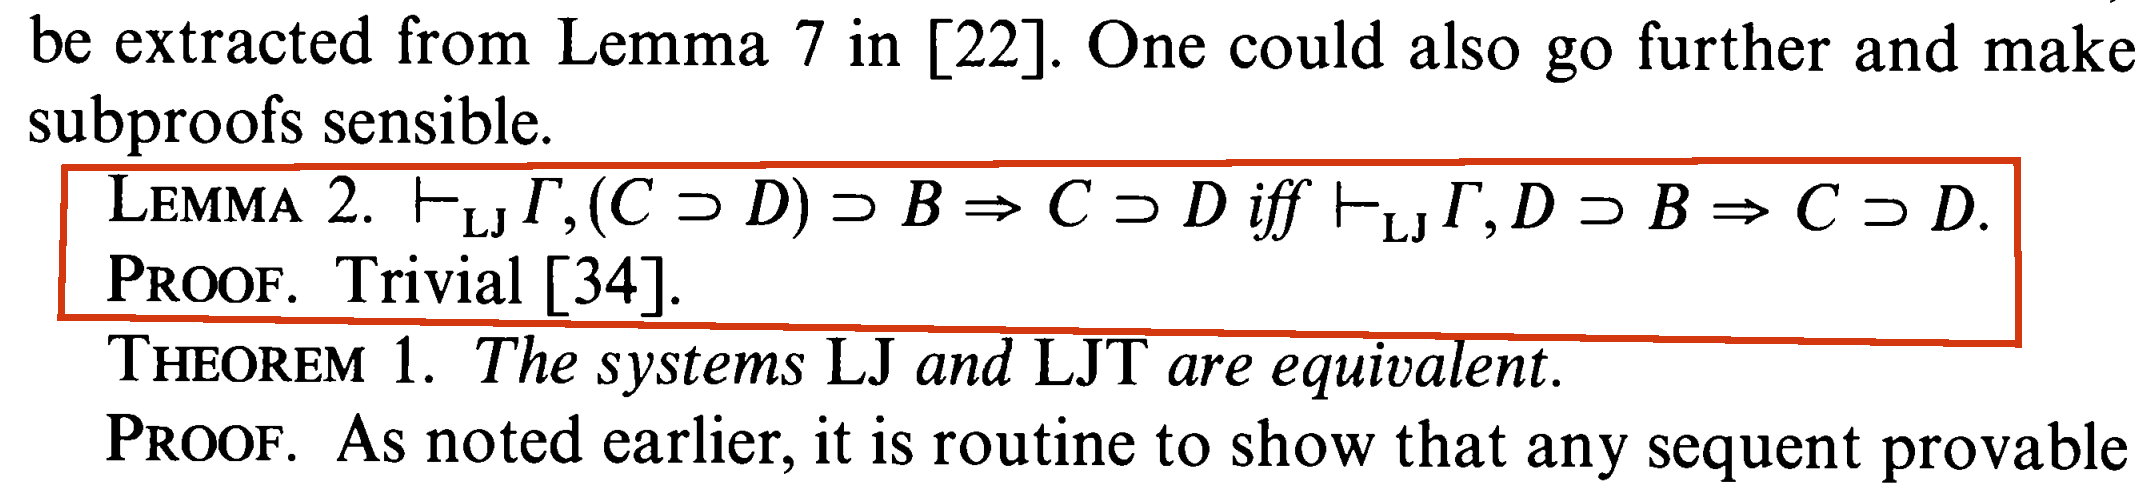
\includegraphics[width=0.8\textwidth]{Vorobieff-lemma}
\par\end{center}

\begin{center}
{\footnotesize{}{[}R. Dyckhoff, }\emph{\footnotesize{}Contraction-Free
Sequent Calculi for Intuitionistic Logic}{\footnotesize{}, 1992{]}}{\footnotesize\par}
\par\end{center}

A stepping stone to this theorem:{\footnotesize{}
\[
\left(\left(A\Rightarrow B\right)\Rightarrow C\right)\Rightarrow B\Rightarrow C
\]
}Proof (\emph{obviously} trivial): $f^{\left(A\Rightarrow B\right)\Rightarrow C}\Rightarrow b^{B}\Rightarrow f\:(x^{A}\Rightarrow b)$

\emph{Details are left as exercise for the reader}

Proof search V: From deduction rules to code

The new rules are equivalent to the old rules, therefore...

Proof of a sequent $A,B,C\vdash G$ $\Leftrightarrow$ code/expression
$t(a,b,c):G$

Also can be seen as a function $t$ from $A,B,C$ to $G$

Sequent in a proof follows from an axiom or from a transforming rule

The two axioms are fixed expressions, $x^{A}\Rightarrow x$ and $1$

Each rule has a \emph{proof transformer} function: $\text{PT}_{R\Rightarrow}$
, $\text{PT}_{L+}$ , etc.

Examples of proof transformer functions:
\begin{align*}
\frac{\Gamma,A\vdash C\quad\;\Gamma,B\vdash C}{\Gamma,{\color{blue}A+B}\vdash C}\:L+\\
PT_{L+}(t_{1}^{A\Rightarrow C},t_{2}^{B\Rightarrow C})=x^{A+B}\Rightarrow & \ x\ \text{match}\begin{cases}
a^{A}\Rightarrow t_{1}(a)\\
b^{B}\Rightarrow t_{2}(b)
\end{cases}
\end{align*}
\begin{align*}
\frac{\Gamma,A\Rightarrow B\Rightarrow C\vdash D}{\Gamma,{\color{blue}(A\times B)\Rightarrow C}\vdash D}\:L\Rightarrow_{2}\\
PT_{L\Rightarrow_{2}}(f^{\left(A\Rightarrow B\Rightarrow C\right)\Rightarrow D})=g^{A\times B\Rightarrow C}\Rightarrow & f\,(x^{A}\Rightarrow y^{B}\Rightarrow g(x,y))
\end{align*}

Verify that we can indeed produce PTs for every rule of LJT

Proof search example II: deriving code

Once a proof tree is found, start from leaves and apply PTs

For each sequent $S_{i}$, this will derive a \textbf{proof expression}
$t_{i}$

Example: to prove $S_{0}$, start from $S_{6}$ backwards:{\footnotesize{}
\begin{align*}
S_{6}:\left(R\Rightarrow R\right)\Rightarrow Q;R\vdash R\quad(\text{axiom }Id)\quad & t_{6}(rrq,r)=r\\
S_{2}:\left(R\Rightarrow R\right)\Rightarrow Q\vdash\left(R\Rightarrow R\right)\quad\text{PT}_{R\Rightarrow}(t_{6})\quad & t_{2}(rrq)=\left(r\Rightarrow t_{6}(rrq,r)\right)\\
S_{3}:Q\vdash Q\quad(\text{axiom }Id)\quad & t_{3}(q)=q\\
S_{1}:\left(R\Rightarrow R\right)\Rightarrow Q\vdash Q\quad\text{PT}_{L\Rightarrow}(t_{2},t_{3})\quad & t_{1}(rrq)=t_{3}(rrq(t_{2}(rrq)))\\
S_{0}:\emptyset\vdash\left(\left(R\Rightarrow R\right)\Rightarrow Q\right)\Rightarrow Q\quad\text{PT}_{R\Rightarrow}(t_{1})\quad & t_{0}=\left(rrq\Rightarrow t_{1}(rrq)\right)
\end{align*}
}{\footnotesize\par}

The proof expression for $S_{0}$ is then obtained as
\begin{align*}
t_{0} & =rrq\Rightarrow t_{3}\left(rrq\left(t_{2}\left(rrq\right)\right)\right)=rrq\Rightarrow rrq(r\Rightarrow t_{6}\left(rrq,r\right)\\
 & =rrq\Rightarrow rrq\left(r\Rightarrow r\right)
\end{align*}
Simplified final code having the required type: 
\[
t_{0}:\left(\left(R\Rightarrow R\right)\Rightarrow Q\right)\Rightarrow Q=\left(rrq\Rightarrow rrq\left(r\Rightarrow r\right)\right)
\]


\section{Intuitionistic propositional logic (IPL)}

The intuitionistic propositional logic (sometimes also called the
``constructive'' propositional logic) describes how programs in
functional programming languages may be able to compute values of
different types.

The main formal difference between IPL and the classical (Boolean)
logic is that IPL does not include the axiom of excluded middle (``\emph{tertium
non datur}''), which is 
\[
\forall A:(A\text{\emph{ or}}\left(\text{\emph{not}}\left(A\right)\right))\text{ is true}\quad.
\]
However, given just this information, it is not easy to understand
the consequences of \emph{not having} this axiom, or to figure out
which statements are true in the IPL. 

The reason this axiom is not included in IPL is that IPL propositions
such as ${\cal CH}(A)$ correspond to the \emph{practical possibility}
of values of type $A$ \emph{to be computed} by a program. For the
proposition ${\cal CH}(A)$ to be true in IPL, a program needs to
actually compute a value of type $A$. It is not sufficient merely
to show that the non-existence of such a value would be somehow contradictory.
But in classical logic, the axiom of excluded middle says that either
${\cal CH}(A)$ or $\text{\emph{not}}\left({\cal CH}(A)\right)$ is
true. So showing that ``$\text{\emph{not}}\left({\cal CH}(A)\right)$''
is contradictory is sufficient for proving ${\cal CH}(A)$, without
ever computing any values of type $A$. For this reason, classical
(Boolean) logic does not adequately describe the logic of types in
functional programming, i.e.~it does not correctly predict the types
of values that can be computed by functional programs.

\section{Example: The logic of types is not Boolean}

Here is an explicit example of obtaining an incorrect result when
using classical logic to reason about values computed by functional
programs. Consider the formula
\begin{equation}
\left(A\Rightarrow B+C\right)\Rightarrow\left(A\Rightarrow B\right)+\left(A\Rightarrow C\right)\label{eq:abc-example-classical-logic}
\end{equation}
or, putting in all the parentheses for clarity,
\[
\left(A\Rightarrow\left(B+C\right)\right)\Rightarrow\left(\left(A\Rightarrow B\right)+\left(A\Rightarrow C\right)\right)\quad.
\]
This formula is a true theorem in classical logic. 

In the IPL, it turns out that Eq.~(\ref{eq:abc-example-classical-logic})
is not a valid theorem, i.e.~it is impossible to find a proof of
Eq.~(\ref{eq:abc-example-classical-logic}) using the axioms and
the derivation rules of the IPL. To \emph{prove} that there is no
proof, one needs to use methods of proof theory that are beyond the
scope of this book. A good introduction to the required technique
is the book ``\emph{Proof and Disproof in Formal Logic}'' by R.~Bornat.\footnote{~\href{https://www.amazon.com/Proof-Disproof-Formal-Logic-Introduction/dp/0198530277}{R. Bornat, "Proof and Disproof in Formal Logic", Oxford, 2005 - link to Amazon.com}} 

This example illustrates that it is precisely the valid theorems in
the IPL, and not the valid theorems in the Boolean logic, that correspond
to implementable functional programs.

\section{Using truth values in Boolean logic and in IPL}

Another significant difference between IPL and the Boolean logic is
that propositions in IPL cannot be assigned a fixed set of ``truth
values''. This was proved by G�del in 1935. It means that a proposition
in IPL cannot be decided by writing out a truth table, even if we
allow more than two truth values.

\begin{comment}
so suppose we we know we need this type how do we get this code turns
out mathematicians have studied this question for a long time mathematicians
were only studying the logical domain of course not the program in
domain since about 1930 or so many mathematicians have studied this
including church tarski girdle lots of people in Poland and Germany
in England and in the United States it took a very long time about
50 years between 1913 and 1980 between the beginning of this activity
when this was first formulated as logic with these particular rules
and the time when the Curie Howard respondents was realized that or
was it wasn't was discovered at that time it became clear that these
things have a direct bearing on functional programming actually helping
people to write code because if you know how to prove things here
you just directly write the code

~

showing here this is equivalent in Scala just different syntax importantly
non theorems cannot be implemented in code some on theorems are statements
in logic that cannot be derived statements that are false or undereye
verbal examples of these statements are these for all a from one follows
a now this is certainly suspicious in terms of logic what if a were
false then we would have it from true false false that's very obviously
wrong and we cannot implement a function of this type to implement
it we would have to take a unit argument and produce a value of type
a where a is arbitrary type but how can we produce a value of type
a of the type that we don't even know what it is and there is no data
for us to produce that value so it is impossible another example of
an impossible type is this type so from a plus B follows a if you
wanted to implement this function you would have to take a value of
disjunction type a plus B and return a value of type a but how can
you do that what exodus Junction type happens to contain B and no
a just B it cannot contain a if it contains a B it's a disjunction
so then we don't have an A and then we again cannot produce any and
having a B which is a completely different arbitrary type doesn't
help us to produce me exactly the same reason shows why we cannot
produce an A a and B given a because that requires a B we cannot produce
and also this is not implementable because we are required to produce
an A but all we have is a function from A to B this function will
consume an A if given only this function cannot possibly produce an
A for us but we are required to produce an A as a result so we cannot
and also there is no proof of this formula in the logic so these examples
actually lead us to a natural question how can we decide given a certain
formula whether it is a theorem in logic and therefore whether it
can be implemented in code it is not obvious consider this example
can we write a function with this type in Scala it is not obvious
can we prove this formula it is not clear not quite obvious right
now suppose I were of the opinion that this cannot be proved but how
do I show that this cannot be proved I certainly cannot just try all
possible proofs that would be infinitely many possible proofs that
would give me all kinds of other formulas and that would give me nothing
that I can stand oh how to answer these questions so it is really
a very hard question we are not going to try to answer it on our own
we were going to use the results of mathematicians they have studied
these questions for many many years for centuries logic has been studied
since ancient Greece more than 2,000 years of study all we need to
do is to find out by what name mathematicians call this logic they
are probably already studied it what kind of logic is this that we
are using that follows from the type constructions remember and the
very beginning of our consideration we started with the type constructions
that our programming languages have so that's set of type constructions
specifies the set of rules of derivation of the logic mathematicians
call this logic intuitionistic propositional logic or IPL also they
call it constructive propositional logic but it is less frequently
used most frequently used name is this and mathematicians also call
this a non classical logic because this logic is actually different
from the boolean logic that we are familiar with the logic of the
values true and false and their truth tables I assume that you are
familiar with those computations using truth tables and operations
and or not in the boolean logic so actually this logic the logic of
types as I call it or intuitionistic propositional logic is very different
from boolean logic in certain ways it's similar in other ways disjunction
for instance works very differently here's an example consider this
sequence if it has given that from a follows B plus C then either
from a follows B or from a follows C it sounds right from the common-sense
point of it if if B plus C Falls a B or C if I was I'm using plus
as a logical or so if B or C follows then it kind of makes sense either
B follows or C Falls indeed this is correct in the boolean logic which
we can find out by writing the truth table so we enumerate all the
possibilities for a B and C to be true or false or eight such possibilities
and for each of those possibilities we write the truth value of this
the truth value of this and we see from the table that whenever this
is true then this is also true in the boolean logic but this does
not hold in the intuitionistic logic for the logic of types well why
does it not hold that's counterintuitive well in fact there is very
little that's intuitive about this so-called intuitionistic logic
actually we need to think differently about this logic we need to
think can we implement an expression of this sequent so implementing
it would mean if we're given this expression we can build an expression
of this type so we're given an expression of type A to B plus C let's
say some F of this type can we build an expression of this type we
can this differently by asking can we implement a function that takes
this as an argument and returns this well we know that this is equivalent
one of our derivation rules is that if you have this sequence then
you can also have a sequence that is a function type from this to
this so for the programmer it is easier to reason about a function
taking this as an argument and returning this so how can we implement
this function this function takes F and needs to return a value of
this type so the body of this function if we could implement it and
have to construct a value of type either of something there are only
two ways of constructing a value of type either one is to construct
the left value second is to construct the right value how do we decide
whether to construct the left value or the right value we have to
decide it somehow on the basis of what information can we decide it
we don't actually have any such information what we have here is a
function from a to either BC so given some value of a of type a we
could compute f of that value and then we would have either B or C
we could decide them whether to we could take them that B or that
C but that's not what we need to return we don't need to return either
of BC we need to return either of this function or that function and
that function is not yet applied to any a it is it is too late for
us to ask what is the a we already have to return the left of this
or a right of that in other words this type either of something-something
is not itself a function of a it contains functions away but itself
it cannot be decided on the basis of any assets too late so we need
to supply a left or right so here right away immediately we have to
decide whether this will return a left or a right and we cannot really
decide that if we decide we return the left we must then return a
function from A to B so there's no way for us to construct this function
if we're given this function because this function could sometimes
return C instead of B and then we'll be stuck we cannot do this and
we can also return we cannot also return the right either so it is
impossible to implement a function of this type implication also works
a little differently in the intuitionistic logic here's an example
this holds in boolean logic but not in intuitionistic logic again
let's see why how can we compute this given this this function will
give us an e only when given an argument of this type but how can
we produce a value of this type we cannot we don't have information
that will allow us to produce a value of this type a and B are some
arbitrary types remember there is universal quantifier outside of
all this for all a and for all B we're supposed to produce this and
that is impossible we don't have enough data to produce some values
type a and so we cannot implement this function conjunction works
kind of the same as in boolean logic so here's an example this implemented
and this is also in boolean logic a true theorem now in boolean logic
the usual way of deciding whether something is true or something is
a theorem is to write a truth table unfortunately the intuitionistic
logic cannot have a truth table it cannot have a fixed number of truth
values even if you allow more than two truth values such that the
validity of formulas the truth of theorems can be decided on the basis
of the truth table this was shown by noodle and this means we should
not actually try to reason about this logic using truth values it
is not very useful even an infinite infinite number of truth values
will not help instead however it turns out that this logic has a decision
procedure or an algorithm and this algorithm is guaranteed either
to find the proof for any given formula of the internation intuitionistic
logic or to determine that there is no proof for that formula the
algorithm can also find several in equivalent proofs if there is a
theorem so a theorem could have several in equivalent proofs and since
each proof could be automatically translated into code of that type
it means we could generate several in equivalent expressions of some
type sometimes so that is the situation with this logic which we discover
if we write if we read papers about intuitionistic propositional logic
that are available in the literature and their open source projects
on the web such as the gen GHC which is a compiler plugin for haskell
this is another project doing the same thing and for Scala are implemented
occurred the Clary Howard library both of these Scala and Haskell
all of these color and Haskell projects do the same thing they take
a type of some expression for function and generate code for it automatic
by translating the type into sequence finding a proof in this logic
using the algorithm and translating that proof back into code in the
way that we have seen in an example it is interesting that all these
provers and there's a few others there's one more for the idris language
I did not mention here they all used the same decision procedure or
the same basic algorithm which is called ljt which was explained in
a paper by dick off here they all side the same paper and I believe
this is so because most other papers on this subject are unreadable
to non-specialists they are written in a very complicated way or they
describe algorithms that are too complicated so I will show how this
works in the rest of this tutorial in order to find out how to get
an algorithm we need to ask well first of all do we have the rules
of derivation that allow us to create an algorithm already here is
a summary of the axioms and the rules of derivation that we have found
so far these are direct translations of the cold expressions that
we held in the programming language in the notation of sequence now
there's one other notation for derivation rules which looks like a
fraction like this the numerator is one or more sequins and the denominator
is a sequence and this notation means in order to derive what is in
the denominator you have to present proofs for what is in the numerator
so this is the convention in the literature this fraction like syntax
or notation now we keep in mind that proofs of sequence are actually
just called expressions that have these types as some variables and
this type is the entire expression so these are directly responding
to proofs of this sequence and to the proofs of these derivation rules
and so if we have a proof that operates by combining some of these
axioms and some of these generation rules which directly translate
that back into code now the question is do these rules give us an
algorithm for finding a proof the answer is no how can we use these
rules to obtain an algorithm well suppose we need to prove some sequence
like this in order to prove it we could first see if the sequence
is one of the axioms if so then we have already proved if we know
what expression to write now in this case none of the axioms match
this so much means maybe a is a times B so B here is C and then on
the Left we must have C or you must have a times B now we don't you
don't have C on the left as we have because even that's not the same
we also don't have a times B at the premise we have a but we don't
have a times B so these rules don't match the other rules don't match
the premises and the goal either but also these rules so how can we
use them well when the writer must be an implication we don't have
an application on the right here we could try to delete some of the
premises because it's unused well actually it doesn't look like a
good idea could you read a for example and we end up with an really
hopeless sequence from B plus C we cannot get an A ever and so but
sounds hopeless so this doesn't seem to help and changing the order
doesn't seem to help much either and so we cannot find matching rules
but actually this sequence is provable just a clever combination of
what axiom to start with and what role to use and then again some
axiom and so on it will give us that time sure because I know how
to write code for this this is not difficult you have a function with
two arguments one of them is a the other is B plus C so disjunction
of either B C and we are supposed to produce a disjunction of tuple
a B or C that's easy look at this disjunction if we have a B in this
disjunction then we can produce a left of the tuple a B because we
always have an A anyway if we have a see in this disjunction then
we could return this part of the disjunction in the right of C and
we're done but unfortunately we see that the rules here do not give
us an algorithm for deciding this we need a better formulation of
the logic again mathematicians need to save us from the situation
and they have done so mathematicians have studied this logic for a
long time starting from the early 20th of the last century the first
algorithmic formulation of the logic that was found is due to Jensen
who published what he called the calculus just ignore the word calculus
it means not very much complete and sound calculus means that he came
up with some rules of derivation which are summarized here such that
they are equivalent to these they derive all the same theorems and
only the same theorems so they derive all the stuff that is right
and only that stuff they don't derive any wrong statements it's very
hard to come up with such a system of axioms and derivation rules
that are equivalent to another one in this sense also it's very hard
to prove that these are actually the rules that will give you all
the theorems that could be right in this logic that you can actually
derive all the theorems that are right yet work is already done by
mathematicians so we're not going to try to do it ourselves we're
just going to understand how these rules work now the syntax here
is slightly enhanced compared with this the enhancement is that their
names pretty cool now these are just labels they don't really do anything
in terms of sequence these help us identify which we all have has
been applied to which sequence and that's all we do so other than
that it is the same notation so the fraction such as this one means
that there is a sequence in the denominator which we will prove if
there are proofs given for sequence in the numerator in this rule
there are two sequence of them in the numerator other rules may have
one sequence in the numerator or no sequence in the numerator so these
rules that will have no previous sequence required those are axioms
this axiom means if you have an atomic X in other words it's a variable
it's a type variables not not a complicated expression just attack
variable and you can derive that same variable this is our accion
right here now why is it important that this is atomic that this is
type variable and not a more complicated expression actually not important
but it's the simplest rule that you can come up with and mathematicians
always like the most minimal set of rules so that's why they say let's
only consider this rule for the type variables X not for more complicated
expressions but we can consider this rule for any expression of course
the identity axiom well here is a truth truth axiom net which derives
the truth which is the ste symbol which I denote it by one the format
in logical notation this is the T symbol well let's just call this
one for clarity so that can be derived from any premises with no previous
sequence necessary none of these other rules now what do these other
rules do they do an interesting thing actually each of these rules
is either about something in the sequence on the left to the trans
time or something in the sequence to the right of the transplant which
I here shown in blue so these are the interesting parts of the sequence
that are being worked on or transformed by the rule so here's an example
this rule is actually two rules the eyes the index so I is one or
two another two rules just written for gravity like this with index
I and each of them says you will prove this if you prove one of if
you prove this so for example you will prove C given if you're given
a a one A two if you will prove C given just a one which makes sense
because if you can prove C given a one you don't need a two we can
ignore this a T we can already proved C from anyone so in this way
it would be proved and so all these rules work in this way you can
prove what's on the bottom of the seat of the of the fraction if you're
given proofs for what's on the top so these are eight derivation rules
and two axioms we can use this now to make a proof search how do we
do that I start with a sequence we see which rule matches that sequence
so the sequence must have something on the left and something on the
right well at least one of these it cannot be empty so it must be
something somewhere and there are only four kinds of expressions in
our logic type variables conjunctions implications and disjunctions
now notice I'm using this arithmetic arithmetic all notation for logic
just because I like it better and I will show that it has advantages
later so we take a sequence we see which rule matches one of them
won't match because either in the premise we have one of these expressions
were in the goal we have one of these expressions and then we find
the rule of match that matches we apply that rule so we now have new
sequence one or more that we will need to be proved and if they're
true then we fork the tree and now we have to prove both of them son-in
we continue doing that for each of the sequence until we hit axioms
so the tree will and this leaf or we hit a sequence to which no rule
applies in which case we cannot prove it and the entire thing is unprovable
so in the search tree there will be sequence at the nodes of the tree
and proofs will be at the edges of the tree so each node sends its
proof to the root of the tree this calculus is guaranteed by mathematicians
to be such that indeed if you cannot find a rule that applies that
means the sequence cannot be proved which was not the case here the
sequence can be proved and yet we cannot find a rule that applies
so in this calculus we can use bottom-up approach to make a proof
search as a tree here we cannot that is the advantage capitalizing
on the mathematicians results let us look at an example suppose we
want to prove this formula this theorem so first step we need to write
a sequence and this needs to be proved from no premises so we write
a sequence s0 which has an empty set of premises this is a single
now what rule applies to this sequence with your bottom up so in other
words we look at these rules and they refine which denominator matches
our sequential and our cylinders empty set on the left so all the
rules on the left cannot be applied but on the right we have an expression
which is an implication at the top level of this expression there
is this implies that so this is of the form a implies B so this rule
applies we have a sequence of the form something in our case this
is an empty set and then a implies B so we apply this rule which is
the right implication and we get a new sequence which is that what
was here before the implication is now put on the left to the trans
of the to the left of the trans time and it means that this expression
needs to be now to the left of the turnstile so now this is the sequence
s1 now we need to prove s1 well we see what rule applies to us one
well on the right there is just Q so nothing can be done of these
rules and Q is not truth so we cannot use the axiom either so let's
look at their left rules on the Left we have now an implication so
this is let's say a and this is B so we have a rule which has a implication
B on the left this is the row left implication let's apply it that
law will give us two new sequence so these two new sequence are s2
and s3 no these ones as you can check if you match a location B against
this implication Q so this is a this is B so then you get these two
sequence now we have to prove these two sequence as 2 and s 3 s 3
is easy it is just the axiom of identity it is this now as 2 again
has an implication on the left let's again apply the rule left implication
to that we get two more sequence as foreign s5 as for is this because
5 is this so now actually we are in trouble because as 2 and s 4 is
are the same sequence as 5 actually we could prove with some more
work but that won't help because we are in a situation when to prove
as two we need to prove again s 2 so that's it that's a loop that
will never give us anything it means we applied the wrong rule so
we need to backtrack this step when we apply the rule left implication
to s 2 we erase is 4 in this 5 and try a different rule to apply to
s 2 which rule can apply to s 2 well as to is this it actually has
implication on the right so we can use the right implication rule
and if we do that we get a sequence s 6 which is this and this sequence
immediately follows from the identity axiom because it has promise
are on the left and premise are and goal are on the right and that
is this axiom whatever other premises and the premise X on the left
premise X on the right and that is a type variable so that's perfect
we have done the proof as 6 follows from the axiom and therefore we
have proved s0 no more sequins need to be proved and because sequence
s0 shows this to be derived from no premises than this formula is
the theorem that's what the theorem means in the logic so that is
how we use this calculus to do proof search now we notice that we
were a bit stuck at some point we had a loop now if we are in the
loop we don't know what to do maybe we need to continue applying the
same rule maybe some new sequence come up or maybe we should not continue
it is not clear what to do and just looking at the rule left implication
shows us that it's copying this premise a implication B it is copied
into the premises of the new sequence and so it will generate a loop
assuredly after the second time you apply it however this sequence
might be new so we might need to apply it second time we don't know
that so that is a problem it will do now there have been a lot of
work trying to fix this problem and literally decades from research
by mathematicians the main ones I found were what are the off we published
in the Soviet Union who de Meyer and dick Hoff who published in the
United States over this time discovered gradually a new set of rules
which is called ljt or the calculus ljt which cures this problem of
looping the way it clears this problem is by replacing this rule left
implication through four new rules which are listed here all other
rules are kept the same from this calculus except the rule left implication
which is replaced in what way so left implication was applying it
applied to a sequence when the sequin had an implication among the
premises or on the left to the left of the turnstile the new rules
look in more detail at what is that implication so that implication
could have one of the four expressions as the argument of the implication
it could have an atomic expression as the argument it would have a
conjunction as the argument could have a disjunction as the argument
or it could have an implication as the argument in our logic there
are no more expressions except these four atomic variables conjunctions
disjunction and implications and so we have here enumerated all the
possibilities for what could be to the left of the implication in
this premise which I have here shown in the blue in blue and so for
each of these we do certain things replacing this sequence with one
or more other sequence again it's quite a lot of work to prove that
these rules are equivalent to these and also that the new rules are
somehow better they are not giving loops a lot of work which I am
NOT going to go through because that's far too complicated for the
scope so what we need suffice it to say that we have very smart people
who published on this and it is reasonably sure that this is correct
so the T in the name lgt starts stands for terminating so if we use
these rules in the same way by by creating a proof tree the proof
tree will have no loops and will terminate after a finite number of
steps and there is actually this paper that is also helpful for understanding
how to implement this algorithm and this paper shows explicitly how
to construct an integer function from sequence to integers which is
a measure of the complexity of the sequence and this measure decreases
every time you apply a rule so it strictly decreases and since this
is a strictly decreasing measure on the proof tree it means that all
the next nodes in the proof tree will have a smaller value of this
measure so eventually it will hit zero and the proof tree will terminate
at that leaf either that or you have no more rules to apply and if
you have no more laws to apply then again mathematicians have proved
it means our sequence cannot be proved so this is an important result
that we are going to use and note that this this rule is quite complicated
it does a very interesting thing it takes this expression which has
implication inside an implication and it transforms this expression
in a weird way namely the B here is separated from the C by parenthesis
but here it is not separated so this transformation is highly non-trivial
and unexpected and its validity is based on this theorem that this
in the intuitionistic logic is equivalent to this equivalent means
they're both following from the other so from this promos that and
from there follows this so this key theorem was attributed to rob
you off my dick off in this paper and this is this lemma 2 which says
that if this sorry that the this derivation is if and only if that
derivations will have these two equivalences and the proof is trivial
and the 34 is a reference to to borrow be off now when a mathematician
says that something is trivial doesn't mean that a statement is easy
to understand it doesn't mean that the proof is easy to find or that
it has trees easy to understand it means none of these things it just
means that right now for this mathematician it is not interesting
to talk about how it is done that's all it means could be for any
number of reasons for example mathematicians could just be lazy or
have no time to again explain this and so they say it's trivial don't
be don't be deceived when you see somebody says that something is
trivial in a mathematical text so to prove this one stepping stone
could be to prove this first this is an easier theorem and if you
prove this then clearly from here you can get B to C B to C you can
substitute in here you can get a to B and then you have here a to
B so in this way you can show this equivalence in one direction now
the proof of this statement is obviously trivial in order to show
the expression of this type I will use my short notation so this is
F which has this type the first argument of the function the second
is B which is at this type then we need to produce a see how do we
produce a C we apply F to an argument of this type the argument of
this type is a function that takes a and returns a B so we take some
X of type a and we return a B which was this B so we ignore this X
we just returned that B and that's the argument of F so this expression
is the proof of this sequence in other words this is the code that
has this type and therefore the proof must be available somehow so
the details of proving this theorem are left as an exercise for the
reader again when you see in a mathematical text that something is
left as an exercise for the reader it does not mean that it is easy
to do it does not mean that for you it would be a useful exercise
to do it also does not mean that the author knows how to do it it
means none of these things it just means the author doesn't feel like
doing it right now and showing it to you for whatever reason could
be because they are lazy it could be because I don't know how to do
it could be because they feel that they should know how to do it but
they don't really do know how to do it could be any of these reasons
don't be deceived when you see something like this but of course I
had to actually produce an expression function of this type in order
to implement my curry forward language because as I will show in a
moment we need to be able to implement all these has code in order
to help approver so why is that we believe the mathematicians that
the new rules are equivalent to the old rules which means that if
you find a proof using these rules somehow you should be able to find
the proof also using our initial rules which means that if you found
that proof it would easily translate that to code because each step
here is directly corresponding to a certain code expression as we
have seen at the beginning of this tutorial these cold expressions
from each of these operations so in order to do this with new rules
in other words in order to create code from proof using new rules
we need to show equivalence or we need to show how to get code out
of each of the new rules now proof of a sequence means that we have
some expression let's say T what uses variables a B and C of these
types and expression itself has type G and also as I have shown this
could be conveniently seen as a function the T as a function from
a B and C from these three arguments to the type G so for each sequencing
a proof we should be able to show either that it follows from an axiom
one of these or that it show it follows from a derivation rule and
the derivations all transforms one proof into another the axioms are
just fixed expressions as we had before the axiom that actually didn't
change between our initial formulation of the logic and the new calculus
lgt they actually did not change the derivation rules changed each
new derivation rule means that you're given expressions that prove
the sequence in the numerator one or more and you are out of these
expressions somehow you have to construct an expression that proves
this sequence now when I say an expression proves the sequence what
it means is that expression has the type that is described by the
sequence it's the same thing because we described types of expressions
through sequence and only those sequence that correspond to valid
and existing expressions in the programming language only those sequence
can be proved by the logic this is by construction so now we need
to just find what are these expressions that corresponds to each of
the derivation rules in each rule has a proof transformer function
as I call it and the proof transfer function is explicitly a function
that takes one or more expressions that are in the numerator and converts
that to the expression in the denominator that has this type so it
has an expression as it has an explicit function we need to write
down for each of the derivation rules so let's see how this is done
for these two examples of derivation laws first example have a rule
that says if you want to derive this sequence we need to derive these
two sequence now this sequence represents an expression of type C
which uses an expression of type A plus B so let's represent this
as a function from a plus B to C now we will be able to just ignore
these other premises which are common arguments and all these functions
we just pass them and we don't write them out what is the proof transformer
for this derivation rule the proof transformer for it is a function
that has two arguments t1 which is the proof of this must be a function
of type II to see and t2 which is a proof of this sequence which must
be a function of type B to see now earlier I said that sequence represent
expressions that use certain variables but equivalently we can say
these are functions that take these variables and return these expressions
that's more convenient when you implement this in code so what we
need is a function that takes a to C and B to C and returns a function
from a plus B to C and this is the code that does it we take an argument
of type a plus B and we return a match expression if it's in the left
we applied t1 to that value and we get to see if it's in the right
we apply t2 to that value and we get a C so in any case we get a syllabus
so this is a function from a plus B to C as required another example
is the proof transformer for this rule this rule has one sequence
going to one sequence so in order to transform is proof into this
we need a function that takes argument of type A to B to C to D and
returns a function of type tuple a B going to C to D so here's the
code we take a function f of type A to B to C to D we return a function
that takes a G of this type shown here in blue and return we need
to return a D so how do we get a deal we apply F to a function of
type A to B to C so we create that function out of G X of type a going
to Y of type B going to G of x1 so this is a function of type A to
B to C which is the argument of F as required and the result is of
type D so that is what we write so this kind of code is the proof
transformer for this derivation arrow and we need to produce this
proof transformers for every rule of the calculus lgt and I have done
it because I have implemented the Korea Howard library that uses LG
T so I'll must have done it for each flow this is a bit tedious because
there are many of those rules and you need to implement all this machinery
of passing arguments no matter how many in this gamma which are emitted
from this notation for brevity but in of course in the real code you
have to deal with all that too so let's see how this works on an example
because once the proof tree is found we need to start backwards from
the leaves of the tree back to the root on each step we take the proof
expression apply the proof transformer to ative according to the rule
that was used on that step we get a new proof expression and so on
so for each sequence we will get a proof expression and at the end
we'll have a proof expression for the root sequence and that will
be the answer so I will denote denote by T I the proof expressions
for the sequence s hi so starting from s6 s6 was this sequence in
our proof so I mean yes just just going through the proof example
it was here backwards from a 6 back to a 0 s-six was this it followed
from axiom identity it's proof expression t6 is a function of two
variables these two variables of these two types and this function
just returns the second variable so it's a function of RR q and r
and just denote this by our argued and Garibaldi's types r RQ variable
of this type is hard here so this function is very simple just ignores
the first argument and returns or so that is what the axiom does the
next sequence was as to as to was obtained by rule our implication
or right implication from s 6 so the proof transformer for right implication
let's look at the right implication and see what the proof transformer
must be so we are given this sequence for this expression which is
the function body the function body that uses a variable of type a
somehow out of this we need to produce a function expression that
takes an argument of type a and returns that functional body so this
is the code which is just writing a new argument returning the function
body that was our proof transformer we need to convert function body
into a function so we just write that argument and arrow in the function
body so in our case we need this as a function body and so our t2
is a function of our Q and this function is this the sequence s 3
followed from the axiom and so it was just this function this is just
the identity function then we used the left implication so this was
actually still done in the calculus algae but the same thing works
in the calculus lgt I'm just using algae because it's simpler for
example here proof transformer for the left implication is a little
more complicated and so if you look at it what what does it have to
be it takes these two expressions and returns this expression so it
takes a function from A to B to a and from B to C and it returns a
function from A to B to see how does it do it given a function a to
b you use this to derive a from it then you substitute that a into
the function into B you get a B when you use this to derive see from
that B and that's your C so you use this function a to be twice you
put it in here once and then you get an A and substitute back into
the same function when you get a B then you use that and that's exactly
what the proof transformer does it takes this rrq and it uses it twice
substitutes into it something that was obtained from one of the terms
and then uses the second term on the result so then this is the proof
transformer for the rule left implication the result of the proof
transformation is the proof for the sequence s1 finally we use the
right implication again which is just this function construction and
we get the proof expression for the sequence s0 now this proof expression
is written through these t1 t2 t3 we have to substitute all this back
in order to get the final expression so if we substitute first of
all we find this is our our cubone going to tea one of our cutie one
of our queue is this so we have to put it here now t3 is just identity
so we can just remove that so that gets you riq going to our Q of
T 2 T 2 is less if I have to put it in T 6 is just identity on R so
this is our going to our and so finally you have this expression so
that is the final code that has the required type notice that we have
derived this code completely algorithmic to it there was no guessing
we found which rules applied to the sequence with transformed sequence
according to the rules once we found the proof which was if we use
the calculus ljt the proof will be just a finite tree with no loops
it will terminate you can get an exhaustive depth-first search for
it for example and you find all the possible proofs if you want as
well well you will find many in any case in some for some expressions
and then we use the proof transformers which are fixed functions that
you can upfront compute for each these expressions are proof transformers
applied to the previous proofs so these are completely fixed algorithmically
fixed so we have derived this code completely algorithmically given
this expression this type so it is in this way that the career Howard
correspondence allows us to derive the code of functions from there
type signatures another important application of the correspondence
is to analyze type by some morphisms or type equivalences and I was
led to this by asking the question so in this logic or in the types
are these operations plus and times as I denoted them more like logic
more like the disjunction and conjunction or are they more like arithmetic
plus and times because this is kind of not so clear right away our
logic is this intuitionistic logic it in any case this is different
from boolean logic so what are the properties of these types really
so are the properties such that it is better to think about these
operations as plus and times rather than logical conjunction and disjunction
can answer this question I looked at identities that we have in the
water these are some identities from simple ones obvious ones to less
obvious identities like this the equal sign here stands for implication
in both directions so both this implies that and vice versa because
of this each of the implications means a function so since these are
all identities in logic it means that for example the implication
from here to here is a theorem of logic and so it can be implemented
as we know all our identities in logic can be implemented in code
and we even have an algorithm now that can automatically produce proofs
and automatically produce code so that means for any of these identities
that has some ik some expression X on the left and some Y on the right
so some kind of X equals y we have X implies Y and y implies X if
we convert that to code we will have a pair of functions function
from X to one and the function from Y to X what do these functions
do well they convert values in some ways from type X to type Y and
back so do these functions Express the equivalence of the types x
and y so that any value of type X can be converted to some equivalent
value type while and back without any loss of information is that
so that was the question I asked I looked at some examples well first
what does it mean more rigorously that types are equivalent for as
mathematicians say isomorphic the types are isomorphic and we will
use this notation for that if there is a one-to-one correspondence
between the sets of values of these types and in order to demonstrate
that we need a pair of functions one going from A to B the other going
from B to a such that the composition of these functions in both directions
is equal to identity function so F compose G or F value G will give
you from A to B and then from B to a is back so that would be identity
of a to a this will be identity of B to B if this is true if the composition
is identity it means we indeed did not lose any information let's
consider an example this is an identity in the logic a conjunction
with one is equal to a in Scala the types responding to the left and
the right hand sides of this conjunction all of this are equivalent
are the conjunction of a and unit and a itself now we need functions
with these types indeed we can write functions is having these types
a pair of a and unit we need to produce an a out of that we'll just
take the first element of the pair you are done take an X of type
a will produce tuple of a and unit very easy just put a unit value
in the tuple in here done and it's easy to verify that composition
of these functions will not change any values so it will be identity
in both directions another example this is an identity in logic if
this is understood as a disjunction one or a or true or a is true
that is an identity in logic for theorem in the logic are the types
equivalent though the type for 1 plus a is the option in Scala it
is option in Haskell at is called maybe this type is standard library
type in pretty much every functional programming language now option
of a is a disjunction of one or unit and a it is certainly not equivalent
to just unit because this type could contain a value of a in it but
this could not so there is no way that you could transform this type
to this and then back without losing information you could transform
so since this is a theorem you have functions from this type to this
type and back some functions you have them but these functions do
not compose to identity they cannot because what if you had a here
you must map it into unit from this unit back you must map into this
unit you cannot get an a out of unit and so that will erase this information
and that cannot become isomorphism so we see that some logic identities
do yield isomorphism types but others do not why is that let's look
at some more examples to figure out why in all these examples we can
implement functions F 1 and F 2 between the two sets to two types
in both directions and then we can check we certainly can implement
them because these are logical identities but then we can check if
the compositions are identity functions and if so the types are isomorphic
but we find that in the first three examples we can do it but in this
last example we can note now I have written the logical identities
logical theorems with the arithmetic notation I call this arithmetical
notation because this suggests arithmetic operations plus and times
and if you look at these identities this looks like a well-known algebraic
identity from the school algebra in this too but this certainly seen
your own as an arithmetic as an as an arithmetic identity this is
certainly not true in arithmetic it is true in logical if you replace
this with disjunction and this with conjunction this is an identity
in logic so this suggests an interesting thing if you replace disjunction
by plus and conjunction by x and the result is an identity in arithmetic
then it is an isomorphism of types otherwise it is not let's see why
this is so indeed this is so I call this the arithmetic arithmetic
oh very hard correspondence to see how it works let's consider only
the types without loss of generation of generality that have a finite
set of possible values for example a boolean type has only two possible
true and false integer let's say in the computers all the integers
are fine nights ago so those types have a finite set of possible values
and this does not limit our generality because in the computer everything
is finite all types have a finite set of possible values now let's
consider how many values a given type has so that would be the size
of the type or using the mathematical terminology it's called a cardinality
of the type so let's see what is the cardinality of various type constructions
the sum type for example if the cardinality of types a and B is known
and the cardinality of a plus B the sum type the disjunction of a
and B is the sum of the two cardinalities or sizes this is because
a value of the disjunction type is constructed as either a value of
the first part or a value of the second part and so you cannot have
both together and so obviously the different number of values is just
the sum of the two sizes that the number of different values of the
sum type is just the sum of the numbers of different values of types
a and B for the product type again we have an interesting thing it's
the arithmetic product of the sizes of a and B because for every a
value you could have an arbitrary B value so this is a direct product
or transient product of sets and we have school level identities about
the operations plus and times such as these identities or these all
of these identities are valid for arithmetic and they show if you
translate that into statements about the sizes of types they show
that the size of the type on the left is equal to the size of the
type on the right and that is very suggestive in other words if you
take a identity like this and you compute the size of the type on
the left and the size of the type on the right you get an arithmetic
identity of the sizes but you don't get that identity here because
the earth medical formula is not right this is very suggestive if
the sizes are equal and maybe the types are equivalent or isomorphic
when the sizes are not equal then certainly they cannot be equivalent
the function type very interestingly also is described in the same
way it provides the set of all maps between the two sets of values
so for example from integer to boolean that would be all the functions
that take some integer and return some boolean so that's and a number
of boolean values \textasciicircum{} the number of integer values
that's how many different functions you can have as a combinatorial
number so it's an exponential and so the size of the type of function
a to be is the size of the type of B \textasciicircum{} the size of
type of a and again we have all the school identities about powers
and how to multiply powers and so on and they are directly translated
into these three identities if you take the sizes of the types on
the left and on the right the sizes will be equal due to these three
identities since the sizes are equal it's very likely that the type
our actual equivalent so far haven't seen any counter examples to
this in these constructions so this gives us a meaning of the Curie
Howard correspondence so far we have seen three facets of the curly
Howard correspondence one is the correspondence between types and
logical formulas two is the correspondence between code and proofs
and three the correspondence between the cardinality of a type or
the set size of the type and the arithmetic identities that we have
in the school algebra about these types so arithmetical identities
signify type equivalence or isomorphism while logic identities only
talk about how you create some value of this type out of value of
another type so that does not guarantee that it preserves information
it just guarantees that you can implement some function of that type
it doesn't tell you that the function will be an isomorphism so if
one type is logically equivalent to another it means are equally implementable
if one is implementable another is also implementable but no more
than that whereas arithmetical identities actually tell you about
isomorphism of types therefore if you look at types and write them
using my preferred notation which is using the arithmetic all symbols
instead of logical symbols instead of these I'll use these symbols
if I do that this is very suggestive of a possible isomorphism of
types then it becomes very easy for me to reason about types I can
see right away that these two are isomorphic types or that these two
are isomorphic types because I am used to looking at school algebra
it's very obvious then that this is not an isomorphism of types because
this doesn't make sense in the school algebra so reasoning about isomorphic
types is basically school level algebra involving polynomials and
powers so if you are familiar with all these identities as you should
be it will be very easy for you the reason about what types are equivalent
as long as all these types are made up of constants or primitive types
disjunctions tuples or conjunctions and functions which will then
directly be translated into exponential polynomial expressions constants
sums products and expand powers or Exponential's so I call these exponential
polynomial types that is types built up from these type constructions
so all we have been talking about in this tutorial is what I call
exponential polynomial types these are the basic type constructions
that I started with tuple product function exponential disjunction
some unit constant or 1 now just one comment that in the functional
programming community today there is a terminology algebraic types
so people usually call algebraic types the types that are made from
constant types sums and products excluding Exponential's I do not
find this terminology it's very helpful I find it confusing because
what is particularly an algebraic about these identities these are
identities of school algebra the properties of the function type are
described by algebraic identities like this so it would be strange
to call the function type not algebraic whereas these types are algebraic
they are very similar to each other in terms of their properties being
described by identity is known from school algebra so instead of algebraic
types I would prefer to say polynomial types this is much more descriptive
and precise and if you want to talk about function types as well then
you just can you can just say exponential polynomial types or exfoli
types for short so by way of summarizing what we have done so far
what are the practical implications of the career Howard correspondence
so one set of implications is actually for writing code and reason
and eternal code one thing we can do now is if we're given a function
with some type and usually this will be typed with type parameters
all type trainers fully parametric types such as the function we have
been considering here all these functions do not have any types that
are specific like integer or string all the types are fully parametric
and then there are some constructions some type expressions made out
of these types so these are what I call fully parametric functions
for these functions we have a decision procedure an algorithm that
based on the ljt calculus which decides whether this function can
be implemented in code and computer scientists a type is inhabited
if you can produce a value of this type in your program so CH of T
is this proposition which they call type is inhabited and I prefer
to call it just that you can compute a value of this type or code
has the type O code can create a value of this type and so we have
a algorithm that can also generate the code from type when it is possible
if it is not possible the algorithm will tell you so often not always
but often this algorithm can be used actually to generate the code
you want we can also use what I call the arithmetic of glory Harvard
correspondence to reason about type isomorphisms and to transform
types isomorphic we simplify type expressions just like we simplify
expressions in school level algebra by expanding brackets by permuting
the order of terms like a plus B is equal to B plus a or associativity
a times B all times C can be expanded and so on so this allows us
once we have written types in the short notation in the notation that
I prefer which resembles school algebra because it uses the plus and
times symbols instead of the logic symbols so once we rewrite our
types and this notation which I have been doing consistently in this
tutorial it enables us the reason very easily but which types are
equal or isomorphic because we are all familiar with the school level
algebra what are the problems that we cannot solve using this knowledge
one thing we cannot do is to generate code automatically such that
it will be an isomorphism so for instance in an example here we are
able to generate automatically the code of these functions but it
will not be an isomorphism and the lgt algorithm cannot check that
this is nice a morphism that's the important thing this algorithm
does not know about equations or isomorphisms it only knows that it
found some code that has the type you wanted whether this code is
useful to you or not we don't know the algorithm doesn't know this
also if the algorithm finds several such several proofs of a sequence
it will generate several not in equivalent versions of your code it
doesn't know which one is is useful maybe some of them are useless
maybe not the algorithm cannot automatically decide that in general
another thing we cannot do is to express complicated conditions via
types such as that array is sorted the type system is not powerful
enough in all the languages I listed you need a much more powerful
type system such as that in the programming language interests or
add them or cook those are much more powerful type systems that can
express such complicated conditions but for those type systems there
is no algorithm that will generate code another thing we cannot do
is to generate code that has type constructors such as the map function
here's an example in Scala this is a map function on a list so there's
the list of a a is a type parameter and then we say dot map and map
has another type frame to be it takes a function from A to B for any
B so a is fixed but now from any B we can take a function from A to
B and generate a list of B so if we wrote this formula in the short
type notation this would look something like this I'm writing subscript
a because this is a type parameter so this is like an argument or
a type parameter I'm writing it like this and then from this this
is the first argument of the function and then there is a second argument
which is this F and that is another quantifier for B inside parentheses
so this formula has a quantifier inside so far we have been dealing
with formulas that have all quantifiers outside and so we never write
quantifiers explicitly but here we have to write them inside this
is a more powerful logic which is called first-order logic in other
words this is a logic where you have quantifiers anywhere in the formula
including inside the formula unfortunately this logic is undecidable
so there is no algorithm that we can use either to find the proof
and therefore code freedom type or to show that there is no proof
no code so we're kind of stuck in all these directions some more remarks
about the curry Harvard correspondence first is that only with parameterize
types we can get some interesting information out of it if we take
concrete types like integer then the proposition CH event meaning
that our code can have a value of type int it that's always true can
always write any some integer value we don't need any previous data
for it so for all specific types all these propositions are always
choice completely void of information the only interesting part comes
when we start considering type variables if we start asking can we
make a type which is either of a B going to a going to B in soon for
all a B once we start doing this with type parameters a B and so on
then we get interesting information as we have seen in this tutorial
another remark is that functions like this one are not sufficiently
described by their type so that this is the type of integer going
to integer now looking at this type we can put this into a sequence
but we'll never get enough information to actually get this function
so only certain class of functions which are fully typed biometric
their type signature is informative enough so that we can derive code
automatically only in much more powerful type systems you can have
type information that is enough to specify fully a code like this
another caveat is that I don't know the proof that arithmetic identity
guarantees the type equivalence it is certainly a necessary condition
because if two types have different cardinality or different size
of their sets of values that they cannot be equivalent or they cannot
be isomorphic so this is a necessary condition but it's not a sufficient
condition it looks like I don't know if this is sufficient I haven't
seen any counter examples so far final remarks about type correspondence
the logical constant false did not appear in any of my slides so far
this was on purpose it has extremely limited practical use in programming
languages because actually we have types corresponding to false Scala
has type called nothing Haskell has type usually called void that
corresponds to the logical constant false what does it mean CH of
nothing is false it means your code can never have a value of type
nothing or in Haskell void you can never compute a value of this type
so clearly it has a very limited practical significance you will never
be able to compute any values of this type ever in any program it's
identically falseness this constant so if you want to add it to the
logic it's very easy you just have one rule and you're not done you
can derive things with it if you want but they will have almost never
any use in practical code also we did not talk about negation none
of the calculus calculate that I should have in logical negation as
in operation again for the same reason we do not have a programming
language construction that represents logical negation negation by
definition is like this is an application from 8 to 4 so that's not
a not a means from a follows falsehood now since you cannot ever get
false in a programming language you cannot really implement this function
in any useful sense and so i have seen some haskell library that used
this type void as a type parameter in some way but certainly it's
a very limited and rare use and so it is not really lumen 18 to include
negation it could probably find some very esoteric uses of it but
almost never useful and finally there is another set of important
implications from the Kurihara correspondence these are implications
for people who want to design new programming languages as we have
seen the Karaka with correspondence maps the type system of a programming
language into a certain logical system where prepositions follow from
each other or can be proved from each other and this enables us to
reason about programmed to see what kind of code can be written if
some other kind of code can be written and logical reasoning is very
powerful it's simpler than trying to write code and it gives you algorithms
and all kinds of mathematical results that have been found over the
centuries so languages like those listed here have all the five type
constructions that I wasted in the beginning of this tutorial and
mapping them into logic gives a full constructive logic or full intuitionistic
logic with all logical operations and or so conjunction disjunction
implication and the truth constant whereas languages such as C C++
Java and c-sharp and so on they're mapped to incomplete logics because
they do not have some of these operations for instance they do not
have type constructions of correspond to disjunction we also do not
have the true constant or the false constant so they are mapped to
a logic that lacks some of the foundational logical operation so it
can be only fewer theorems can be proved in that logic and so your
reasoning about theory types is hampered languages called scripting
languages sometimes such as Python or JavaScript will be and so on
also our belongs there in that line those languages only have one
type they actually don't check types at compile time and so they're
mapped to logics with only one proposition those logics are extremely
small in terms of what kind of things you can reason about and so
if you write a program in these languages you are completely unable
to reason at the level of types whereas in these languages you are
able to reason but in a limited way you're not having a complete logic
so this suggests a principle for designing the type system in a new
programming language the first step would be to choose a good and
complete logic that is free of inconsistency mathematicians have studied
all kinds of logics and they are always interested in questions such
as is this logic consistent consistent means you cannot derive false
from true is this logic complete can you derive all things that are
true are there enough axioms and rules of derivation or maybe there
are too many axioms and rules of derivation you can delete some of
them and have fewer mathematicians have always been interested in
such questions they found all kinds of interesting logics where you
can derive a lot of interesting theorems non trivial theorems and
they found the minimum sets of axioms and rules of derivations for
these logics use their results take one of the logics that they do
them and develop such as intuitionistic logic model logic temporal
logic linear logic and so on take one of these logics for each of
the basic operations of this logic provide type constructions in your
programming language that are easy to use for instance your logic
has disjunction implication or something else provide a type constructor
for each of them that's easy to use easy to write down such as provided
by the languages we have seen then every type will be mapped to a
logical form of the OPF logical formula for every type and there will
be a type for every logical formula and then for each rule of the
new logic for each derivation rule there should be a construct in
the code that corresponds to it so that you could transform proofs
in logic into code and code into proofs if you do that your language
will be faithful to the scorecard correspondence you will be able
to use logic to reason about your language and one important result
at this level while we have seen that you can sometimes generate code
that is maybe nice but a very important result is that if your logic
is free of inconsistency it means that no program will ever be able
to derive an inconsistent an inconsistent type means that you had
a function that requires some type a but it was called with a different
type beam which is incompatible and that basically crashes so in languages
like C and C++ we have all kinds of crashes like a segmentation fault
in Java the exceptions nullpointerexception or class cast exception
which happens when you call a function on the wrong type of argument
and that happens if your logic is inconsistent if your logic can derive
incorrect statements from correct premises then if you translate that
derivation into code and the that code will derive incompatible type
at the wrong place and it will crash the crash will happen at runtime
the compiler will not catch this inconsistency because the compiler
only checks the logic of types and the logic checks out you have followed
the rules of derivation of the logic the compiler can check out all
these logical rules but the compiler does not know that your logic
is inconsistent maybe and then it will deep have derived an inconsistent
result falsehood from truth for example and that will crash at runtime
now we know that crashing at runtime is not a good outcome so in fact
languages like Oh camel have been studied and for other languages
some subsets of Haskell I believe called safe Haskell have been studied
and it has been shown that they cannot crash and they're the way to
show it mathematically is to use the fact that they are based on a
complete and consistent logic and then all you need to show is that
your compiler does not have some critical bugs that allow it to oversee
that you have not followed the derivation rules of the logic that
is an extremely valuable feature of functional programming languages
that are based on the Curie habit correspondence you can prove their
safety at compile time or at least exclude a large number of possible
bugs and errors certainly these languages are quite large and they
include features that are not covered by the Carey Hart correspondence
type constructors that I have not considered in this tutorial and
those might may not be safe but at least the foundation of these languages
the foundation of the type system will be safe so that is the final
lesson from the great Howard correspondence this concludes the tutorial 
\end{comment}


\chapter{Category theory}

Examples of categories
\begin{enumerate}
\item Objects: types $\text{Int}$, $\text{String}$, ...; morphisms (arrows)
are functions $\text{Int}\rightarrow\text{String}$ etc. \textendash{}
this is the ``standard'' category corresponding to a given programming
language
\item Objects: types $A$, $B$, ...; morphisms are pairs of functions $\left(A\rightarrow B\right),\left(B\rightarrow A\right)$
\item {*} Objects: types $\text{List}^{A}$, $\text{List}^{B}$, ...; morphisms
are functions of type $\text{List}^{A}\rightarrow\text{List}^{B}$
\item Objects: types $A$, $B$, ...; morphisms are functions of type $\text{List}^{A}\rightarrow\text{List}^{B}$
\item Objects: types $A$, $B$, ...; morphisms are functions of type $A\rightarrow\text{List}^{B}$
\item {*} Objects: types $\text{List}^{A}$, $\text{List}^{B}$, ...; morphisms
are functions $A\rightarrow B$
\item Objects: types $A$, $B$, ...; morphisms are $\text{List}^{A\rightarrow B}$
\item Objects: types $A,$ $B$, ...; morphisms are functions $B\rightarrow A$
\item {*} Objects: things $A,$ $B$, ...; morphisms are pairs $\left(A,B\right)$
of things \textendash{} this is the same as a preorder
\end{enumerate}
Examples marked with {*} are for illustration only, they are probably
not very useful

\chapter{A humorous disclaimer}

\emph{The following text is quoted in part from an anonymous source
(``Project Guten Tag'') dating back at least to 1997. The original
text is no longer available on the Internet.}

\medskip{}

\noun{Warranto Limitensis; Disclamatantus Damagensis}

Solus exceptus ``Rectum Replacator Refundiens'' describitus ecci,
\begin{enumerate}
\item Projectus (etque nunquam partum quis hic etext remitibus cum \noun{Project
Guten Tag}-tm identificator) disclamabat omni liabilitus tuus damagensis,
pecuniensisque, includibantus pecunia legalitus, et 
\item \noun{Remedia Negligentitia Non Habet Tuus, Warrantus Destructi\-bus
Contractus Nullibus Ni Liabilitus Sumus, Inclutatibus Non Limitatus
Destructio Directibus, Consequentius, Punitio, O Incidentus, Non Sunt
Si Nos Notificat Vobis}. 
\end{enumerate}
Sit discubriatus defectus en etextum sic entram diariam noventam recibidio,
pecuniam tuum refundatorium receptorus posset, sic scribatis vendor.
Sit veniabat medium physicalis, vobis idem reternat et replacator
possit copius. Sit venitabat electronicabilis, sic viri datus chansus
segundibus. 

\noun{Hic Etext Venid ``Como-asi''. Nihil Warranti Nunquam Classum,
Expressito Ni Implicato, Le Macchen Como Si Etexto Bene Sit O Il Medio
Bene Sit, Inclutat Et Non Limitat Warranti Mercatensis, Appropriatensis
Purposem. }

Statuen varias non permitatent disclamabaris ni warranti implicatoren
ni exclusioni limitatio damagaren consequentialis, ecco lo qua disclamatori
exclusato\-rique non vobis applicant, et potat optia alia legali.

\chapter{GNU Free Documentation License\label{sec:GFDL} }

{\tiny{}Version 1.2, November 2002}{\tiny\par}

{\tiny{}Copyright (c) 2000,2001,2002 Free Software Foundation, Inc.
59 Temple Place, Suite 330, Boston, MA 02111-1307, USA}{\tiny\par}

{\tiny{}Everyone is permitted to copy and distribute verbatim copies
of this license document, but changing it is not allowed.}{\tiny\par}

{\tiny{}\setcounter{subsection}{-1}}{\tiny\par}

\subsection*{{\tiny{}Preamble}}

{\tiny{}The purpose of this License is to make a manual, textbook,
or other functional and useful document free in the sense of freedom:
to assure everyone the effective freedom to copy and redistribute
it, with or without modifying it, either commercially or noncommercially.
Secondarily, this License preserves for the author and publisher a
way to get credit for their work, while not being considered responsible
for modifications made by others.}{\tiny\par}

{\tiny{}This License is a kind of \textquotedblleft copyleft'', which
means that derivative works of the document must themselves be free
in the same sense. It complements the GNU General Public License,
which is a copyleft license designed for free software.}{\tiny\par}

{\tiny{}We have designed this License in order to use it for manuals
for free software, because free software needs free documentation:
a free program should come with manuals providing the same freedoms
that the software does. But this License is not limited to software
manuals; it can be used for any textual work, regardless of subject
matter or whether it is published as a printed book. We recommend
this License principally for works whose purpose is instruction or
reference.}{\tiny\par}

\subsection{Applicability and definitions\label{subsec:1Applicability-and-definitions}}

{\tiny{}This License applies to any manual or other work, in any medium,
that contains a notice placed by the copyright holder saying it can
be distributed under the terms of this License. Such a notice grants
a world-wide, royalty-free license, unlimited in duration, to use
that work under the conditions stated herein. The \textquotedblleft Document'',
below, refers to any such manual or work. Any member of the public
is a licensee, and is addressed as \textquotedblleft you''. You accept
the license if you copy, modify or distribute the work in a way requiring
permission under copyright law.}{\tiny\par}

{\tiny{}A \textquotedblleft Modified Version'' of the Document means
any work containing the Document or a portion of it, either copied
verbatim, or with modifications and/or translated into another language.}{\tiny\par}

{\tiny{}A \textquotedblleft Secondary Section'' is a named appendix
or a front-matter section of the Document that deals exclusively with
the relationship of the publishers or authors of the Document to the
Document's overall subject (or to related matters) and contains nothing
that could fall directly within that overall subject. (Thus, if the
Document is in part a textbook of mathematics, a Secondary Section
may not explain any mathematics.) The relationship could be a matter
of historical connection with the subject or with related matters,
or of legal, commercial, philosophical, ethical or political position
regarding them.}{\tiny\par}

{\tiny{}The \textquotedblleft Invariant Sections'' are certain Secondary
Sections whose titles are designated, as being those of Invariant
Sections, in the notice that says that the Document is released under
this License. If a section does not fit the above definition of Secondary
then it is not allowed to be designated as Invariant. The Document
may contain zero Invariant Sections. If the Document does not identify
any Invariant Sections then there are none.}{\tiny\par}

{\tiny{}The \textquotedblleft Cover Texts'' are certain short passages
of text that are listed, as Front-Cover Texts or Back-Cover Texts,
in the notice that says that the Document is released under this License.
A Front-Cover Text may be at most 5 words, and a Back-Cover Text may
be at most 25 words.}{\tiny\par}

{\tiny{}A \textquotedblleft Transparent'' copy of the Document means
a machine-readable copy, represented in a format whose specification
is available to the general public, that is suitable for revising
the document straightforwardly with generic text editors or (for images
composed of pixels) generic paint programs or (for drawings) some
widely available drawing editor, and that is suitable for input to
text formatters or for automatic translation to a variety of formats
suitable for input to text formatters. A copy made in an otherwise
Transparent file format whose markup, or absence of markup, has been
arranged to thwart or discourage subsequent modification by readers
is not Transparent. An image format is not Transparent if used for
any substantial amount of text. A copy that is not \textquotedblleft Transparent''
is called \textquotedblleft Opaque''.}{\tiny\par}

{\tiny{}Examples of suitable formats for Transparent copies include
plain ASCII without markup, Texinfo input format, \LaTeX{} input format,
SGML or XML using a publicly available DTD, and standard-conforming
simple HTML, PostScript or PDF designed for human modification. Examples
of transparent image formats include PNG, XCF and JPG. Opaque formats
include proprietary formats that can be read and edited only by proprietary
word processors, SGML or XML for which the DTD and/or processing tools
are not generally available, and the machine-generated HTML, PostScript
or PDF produced by some word processors for output purposes only.}{\tiny\par}

{\tiny{}The ``Title Page'' means, for a printed book, the title
page itself, plus such following pages as are needed to hold, legibly,
the material this License requires to appear in the title page. For
works in formats which do not have any title page as such, \textquotedblleft Title
Page\textquotedblright{} means the text near the most prominent appearance
of the work's title, preceding the beginning of the body of the text.}{\tiny\par}

{\tiny{}A section ``Entitled XYZ'' means a named subunit of the
Document whose title either is precisely XYZ or contains XYZ in parentheses
following text that translates XYZ in another language. (Here XYZ
stands for a specific section name mentioned below, such as \textquotedblleft Acknowledgements\textquotedblright ,
\textquotedblleft Dedications\textquotedblright , \textquotedblleft Endorsements\textquotedblright ,
or \textquotedblleft History\textquotedblright .) To \textquotedblleft Preserve
the Title\textquotedblright{} of such a section when you modify the
Document means that it remains a section \textquotedblleft Entitled
XYZ\textquotedblright{} according to this definition.}{\tiny\par}

{\tiny{}The Document may include Warranty Disclaimers next to the
notice which states that this License applies to the Document. These
Warranty Disclaimers are considered to be included by reference in
this License, but only as regards disclaiming warranties: any other
implication that these Warranty Disclaimers may have is void and has
no effect on the meaning of this License.}{\tiny\par}

\subsection{Verbatim copying\label{subsec:2Verbatim-copying}}

{\tiny{}You may copy and distribute the Document in any medium, either
commercially or noncommercially, provided that this License, the copyright
notices, and the license notice saying this License applies to the
Document are reproduced in all copies, and that you add no other conditions
whatsoever to those of this License. You may not use technical measures
to obstruct or control the reading or further copying of the copies
you make or distribute. However, you may accept compensation in exchange
for copies. If you distribute a large enough number of copies you
must also follow the conditions in section~\ref{subsec:3Copying-in-quantity}.}{\tiny\par}

{\tiny{}You may also lend copies, under the same conditions stated
above, and you may publicly display copies.}{\tiny\par}

\subsection{Copying in quantity\label{subsec:3Copying-in-quantity}}

{\tiny{}If you publish printed copies (or copies in media that commonly
have printed covers) of the Document, numbering more than 100, and
the Document's license notice requires Cover Texts, you must enclose
the copies in covers that carry, clearly and legibly, all these Cover
Texts: Front-Cover Texts on the front cover, and Back-Cover Texts
on the back cover. Both covers must also clearly and legibly identify
you as the publisher of these copies. The front cover must present
the full title with all words of the title equally prominent and visible.
You may add other material on the covers in addition. Copying with
changes limited to the covers, as long as they preserve the title
of the Document and satisfy these conditions, can be treated as verbatim
copying in other respects.}{\tiny\par}

{\tiny{}If the required texts for either cover are too voluminous
to fit legibly, you should put the first ones listed (as many as fit
reasonably) on the actual cover, and continue the rest onto adjacent
pages.}{\tiny\par}

{\tiny{}If you publish or distribute Opaque copies of the Document
numbering more than 100, you must either include a machine-readable
Transparent copy along with each Opaque copy, or state in or with
each Opaque copy a computer-network location from which the general
network-using public has access to download using public-standard
network protocols a complete Transparent copy of the Document, free
of added material. If you use the latter option, you must take reasonably
prudent steps, when you begin distribution of Opaque copies in quantity,
to ensure that this Transparent copy will remain thus accessible at
the stated location until at least one year after the last time you
distribute an Opaque copy (directly or through your agents or retailers)
of that edition to the public.}{\tiny\par}

{\tiny{}It is requested, but not required, that you contact the authors
of the Document well before redistributing any large number of copies,
to give them a chance to provide you with an updated version of the
Document.}{\tiny\par}

\subsection{Modifications\label{subsec:4Modifications}}

{\tiny{}You may copy and distribute a Modified Version of the Document
under the conditions of sections~\ref{subsec:2Verbatim-copying}
and \ref{subsec:3Copying-in-quantity} above, provided that you release
the Modified Version under precisely this License, with the Modified
Version filling the role of the Document, thus licensing distribution
and modification of the Modified Version to whoever possesses a copy
of it. In addition, you must do these things in the Modified Version:}{\tiny\par}

{\tiny{}A. Use in the Title Page (and on the covers, if any) a title
distinct from that of the Document, and from those of previous versions
(which should, if there were any, be listed in the History section
of the Document). You may use the same title as a previous version
if the original publisher of that version gives permission.}{\tiny\par}

{\tiny{}B. List on the Title Page, as authors, one or more persons
or entities responsible for authorship of the modifications in the
Modified Version, together with at least five of the principal authors
of the Document (all of its principal authors, if it has fewer than
five), unless they release you from this requirement.}{\tiny\par}

{\tiny{}C. State on the Title page the name of the publisher of the
Modified Version, as the publisher.}{\tiny\par}

{\tiny{}D. Preserve all the copyright notices of the Document.}{\tiny\par}

{\tiny{}E. Add an appropriate copyright notice for your modifications
adjacent to the other copyright notices.}{\tiny\par}

{\tiny{}F. Include, immediately after the copyright notices, a license
notice giving the public permission to use the Modified Version under
the terms of this License, in the form shown in the Addendum below.}{\tiny\par}

{\tiny{}G. Preserve in that license notice the full lists of Invariant
Sections and required Cover Texts given in the Document's license
notice.}{\tiny\par}

{\tiny{}H. Include an unaltered copy of this License.}{\tiny\par}

{\tiny{}I. Preserve the section Entitled ``History'', Preserve its
Title, and add to it an item stating at least the title, year, new
authors, and publisher of the Modified Version as given on the Title
Page. If there is no section Entitled \textquotedblleft History\textquotedblright{}
in the Document, create one stating the title, year, authors, and
publisher of the Document as given on its Title Page, then add an
item describing the Modified Version as stated in the previous sentence.}{\tiny\par}

{\tiny{}J. Preserve the network location, if any, given in the Document
for public access to a Transparent copy of the Document, and likewise
the network locations given in the Document for previous versions
it was based on. These may be placed in the ``History'' section.
You may omit a network location for a work that was published at least
four years before the Document itself, or if the original publisher
of the version it refers to gives permission.}{\tiny\par}

{\tiny{}K. For any section Entitled ``Acknowledgements'' or ``Dedications'',
Preserve the Title of the section, and preserve in the section all
the substance and tone of each of the contributor acknowledgements
and/or dedications given therein.}{\tiny\par}

{\tiny{}L. Preserve all the Invariant Sections of the Document, unaltered
in their text and in their titles. Section numbers or the equivalent
are not considered part of the section titles.}{\tiny\par}

{\tiny{}M. Delete any section Entitled ``Endorsements''. Such a
section may not be included in the Modified Version.}{\tiny\par}

{\tiny{}N. Do not retitle any existing section to be Entitled ``Endorsements''
or to conflict in title with any Invariant Section.}{\tiny\par}

{\tiny{}O. Preserve any Warranty Disclaimers.}{\tiny\par}

{\tiny{}If the Modified Version includes new front-matter sections
or appendices that qualify as Secondary Sections and contain no material
copied from the Document, you may at your option designate some or
all of these sections as invariant. To do this, add their titles to
the list of Invariant Sections in the Modified Version's license notice.
These titles must be distinct from any other section titles.}{\tiny\par}

{\tiny{}You may add a section Entitled ``Endorsements'', provided
it contains nothing but endorsements of your Modified Version by various
parties \textendash{} for example, statements of peer review or that
the text has been approved by an organization as the authoritative
definition of a standard.}{\tiny\par}

{\tiny{}You may add a passage of up to five words as a Front-Cover
Text, and a passage of up to 25 words as a Back-Cover Text, to the
end of the list of Cover Texts in the Modified Version. Only one passage
of Front-Cover Text and one of Back-Cover Text may be added by (or
through arrangements made by) any one entity. If the Document already
includes a cover text for the same cover, previously added by you
or by arrangement made by the same entity you are acting on behalf
of, you may not add another; but you may replace the old one, on explicit
permission from the previous publisher that added the old one.}{\tiny\par}

{\tiny{}The author(s) and publisher(s) of the Document do not by this
License give permission to use their names for publicity for or to
assert or imply endorsement of any Modified Version.}{\tiny\par}

\subsection*{{\tiny{}Combining documents}}

{\tiny{}You may combine the Document with other documents released
under this License, under the terms defined in section 4 above for
modified versions, provided that you include in the combination all
of the Invariant Sections of all of the original documents, unmodified,
and list them all as Invariant Sections of your combined work in its
license notice, and that you preserve all their Warranty Disclaimers.}{\tiny\par}

{\tiny{}The combined work need only contain one copy of this License,
and multiple identical Invariant Sections may be replaced with a single
copy. If there are multiple Invariant Sections with the same name
but different contents, make the title of each such section unique
by adding at the end of it, in parentheses, the name of the original
author or publisher of that section if known, or else a unique number.
Make the same adjustment to the section titles in the list of Invariant
Sections in the license notice of the combined work.}{\tiny\par}

{\tiny{}In the combination, you must combine any sections Entitled
\textquotedblleft History\textquotedblright{} in the various original
documents, forming one section Entitled \textquotedblleft History\textquotedblright ;
likewise combine any sections Entitled \textquotedblleft Acknowledgements\textquotedblright ,
and any sections Entitled \textquotedblleft Dedications\textquotedblright .
You must delete all sections Entitled \textquotedblleft Endorsements.\textquotedblright{}}{\tiny\par}

\subsection*{{\tiny{}Collections of documents}}

{\tiny{}You may make a collection consisting of the Document and other
documents released under this License, and replace the individual
copies of this License in the various documents with a single copy
that is included in the collection, provided that you follow the rules
of this License for verbatim copying of each of the documents in all
other respects.}{\tiny\par}

{\tiny{}You may extract a single document from such a collection,
and distribute it individually under this License, provided you insert
a copy of this License into the extracted document, and follow this
License in all other respects regarding verbatim copying of that document.}{\tiny\par}

\subsection*{{\tiny{}Aggregation with independent works}}

{\tiny{}A compilation of the Document or its derivatives with other
separate and independent documents or works, in or on a volume of
a storage or distribution medium, is called an \textquotedblleft aggregate\textquotedblright{}
if the copyright resulting from the compilation is not used to limit
the legal rights of the compilation's users beyond what the individual
works permit. When the Document is included an aggregate, this License
does not apply to the other works in the aggregate which are not themselves
derivative works of the Document.}{\tiny\par}

{\tiny{}If the Cover Text requirement of section~\ref{subsec:3Copying-in-quantity}
is applicable to these copies of the Document, then if the Document
is less than one half of the entire aggregate, the Document's Cover
Texts may be placed on covers that bracket the Document within the
aggregate, or the electronic equivalent of covers if the Document
is in electronic form. Otherwise they must appear on printed covers
that bracket the whole aggregate.}{\tiny\par}

\subsection*{{\tiny{}Translation}}

{\tiny{}Translation is considered a kind of modification, so you may
distribute translations of the Document under the terms of section~\ref{subsec:4Modifications}.
Replacing Invariant Sections with translations requires special permission
from their copyright holders, but you may include translations of
some or all Invariant Sections in addition to the original versions
of these Invariant Sections. You may include a translation of this
License, and all the license notices in the Document, and any Warrany
Disclaimers, provided that you also include the original English version
of this License and the original versions of those notices and disclaimers.
In case of a disagreement between the translation and the original
version of this License or a notice or disclaimer, the original version
will prevail.}{\tiny\par}

{\tiny{}If a section in the Document is Entitled \textquotedblleft Acknowledgements\textquotedblright ,
\textquotedblleft Dedications\textquotedblright , or \textquotedblleft History\textquotedblright ,
the requirement (section~\ref{subsec:4Modifications}) to Preserve
its Title (section~\ref{subsec:1Applicability-and-definitions})
will typically require changing the actual title.}{\tiny\par}

\subsection*{{\tiny{}Termination}}

{\tiny{}You may not copy, modify, sublicense, or distribute the Document
except as expressly provided for under this License. Any other attempt
to copy, modify, sublicense or distribute the Document is void, and
will automatically terminate your rights under this License. However,
parties who have received copies, or rights, from you under this License
will not have their licenses terminated so long as such parties remain
in full compliance.}{\tiny\par}

\subsection*{{\tiny{}Future revisions of this license}}

{\tiny{}The Free Software Foundation may publish new, revised versions
of the GNU Free Documentation License from time to time. Such new
versions will be similar in spirit to the present version, but may
differ in detail to address new problems or concerns. See \url{http://www.gnu.org/copyleft/}.}{\tiny\par}

{\tiny{}Each version of the License is given a distinguishing version
number. If the Document specifies that a particular numbered version
of this License \textquotedblleft or any later version\textquotedblright{}
applies to it, you have the option of following the terms and conditions
either of that specified version or of any later version that has
been published (not as a draft) by the Free Software Foundation. If
the Document does not specify a version number of this License, you
may choose any version ever published (not as a draft) by the Free
Software Foundation.}{\tiny\par}

\subsection*{\noun{\tiny{}Addendum}{\tiny{}: How to use this License for your
documents}}

{\tiny{}To use this License in a document you have written, include
a copy of the License in the document and put the following copyright
and license notices just after the title page:}{\tiny\par}

{\tiny{}Copyright (c) <year> <your name>. Permission is granted to
copy, distribute and/or modify this document under the terms of the
GNU Free Documentation License, Version 1.2 or any later version published
by the Free Software Foundation; with no Invariant Sections, no Front-Cover
Texts, and no Back-Cover Texts. A copy of the license is included
in the section entitled \textquotedblleft GNU Free Documentation License\textquotedblright .}{\tiny\par}

{\tiny{}If you have Invariant Sections, Front-Cover Texts and Back-Cover
Texts, replace the \textquotedblleft with...Texts.\textquotedblright{}
line with this:}{\tiny\par}

{\tiny{}with the Invariant Sections being <list their titles>, with
the Front-Cover Texts being <list>, and with the Back-Cover Texts
being <list>.}{\tiny\par}

{\tiny{}If you have Invariant Sections without Cover Texts, or some
other combination of the three, merge those two alternatives to suit
the situation.}{\tiny\par}

{\tiny{}If your document contains nontrivial examples of program code,
we recommend releasing these examples in parallel under your choice
of free software license, such as the GNU General Public License,
to permit their use in free software.}{\tiny\par}

\subsection*{{\tiny{}Copyright }}

{\tiny{}Copyright (c) 2000, 2001, 2002 Free Software Foundation, Inc.
59 Temple Place, Suite 330, Boston, MA 02111-1307, USA}{\tiny\par}

{\tiny{}Everyone is permitted to copy and distribute verbatim copies
of this license document, but changing it is not allowed.}{\tiny\par}
